% ----------------------------------------------------------------------- %
% Arquivo: 04-Resultados.tex
% ----------------------------------------------------------------------- %

\chapter{Projeto e resultados}
\label{cap:resultados}

Neste capítulo será abordado o projeto do conversor Buck \interleaved de dois ramos proposto e, em seguida, apresentado medidas da EMI no conversor e possíveis técnicas aplicáveis para a redução da EMI produzida. 
    
    %%%%%%%%%%%%%%%%%%%%%%%%%%%%%%%%%%%%%%%%%%%%%%%%%%%%%%%%%%%%%%%%%%%
    \section{Projeto do conversor Buck \Interleaved de dois ramos} \label{cap:result_proj}
    %%%%%%%%%%%%%%%%%%%%%%%%%%%%%%%%%%%%%%%%%%%%%%%%%%%%%%%%%%%%%%%%%%%
    
    Para o estudo do conversor proposto, sendo iniciado na disciplina de Eletrônica de Potência I, definiu-se algumas especificações de projeto, conforme \autoref{tab:requisitos_buck}.
        
    \begin{table}[htbp]
        \centering
        \caption{Especificações de projeto do conversor Buck \Interleaved de dois ramos}
        \label{tab:requisitos_buck}
        \begin{tabular}{@{}|m{0.50\textwidth}|m{0.15\textwidth}|m{0.10\textwidth}|@{}}
            \hline
             & Valor & Unid. \\
            \hline
            Tensão de entrada               & 24    & \si{\volt}      \\ \hline
            Tensão de saída                 & 5     & \si{\volt}      \\ \hline
            Variação da tensão de saída     & 1     & \si{\percent}    \\ \hline
            Corrente de saída               & 5     & \si{\ampere}     \\ \hline
            Variação da corrente do indutor & 100   & \si{\percent}    \\ \hline
            Frequência de chaveamento       & 50    & \si{\kilo\hertz} \\ \hline
        \end{tabular}
        \indentedfont[0.84\textwidth]{Elaboração própria (2021)}
    \end{table}
    
    Com essas especificações, torna-se possível calcular os componentes de filtro do conversor, utilizando a \autoref{eq:buck_indutor} e a \autoref{eq:cbi_capacitor}. Assim, é obtido o valor de indutância de \SI{31}{\micro\henry} e uma capacitância de \SI{46}{\micro\farad}. A \autoref{fig:esquematico_cbi} apresenta o esquemático desenvolvido no \textit{software} KiCad para a estrutura proposta. Nesse circuito, foi utilizado o \abreviatura.{CI}{circuito integrado} SG3525 para o acionamento dos transistores e adicionados alguns capacitores de filtro de alta frequência (C3, C4, C5 e C7) como boas práticas no desenvolvimento de um \textit{Layout}. Os indutores em L1 e o indutor L2 foram dispostos de tal forma que posteriormente o circuito pudesse ser adaptado para um conversor 3SSC.
    
    \begin{figure}[H]
    	\centering
    	\caption{Esquemático desenvolvido do CBI de dois ramos}
    	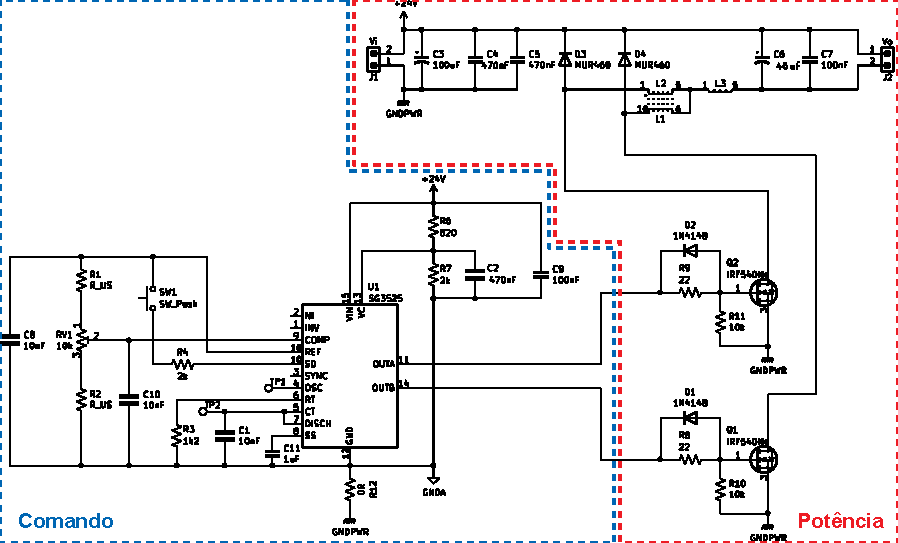
\includegraphics[scale=1]{pdf/layout/Esquematico_CBI_kicad_3.pdf}
        \label{fig:esquematico_cbi}
     	\indentedfont[15.2cm]{Elaboração própria (2021)}
    \end{figure}
    
    Seguido do desenvolvido do esquemático, projetou-se o \textit{layout} da PCB, mostrado na \autoref{fig:layout_cbi}. Durante esse processo, também seguiu-se as boas práticas de desenvolvimento de um \textit{layout} de PCB. 
    
    \begin{figure}[H]
    	\centering
    	\caption{\textit{Layout} desenvolvido do CBI de dois ramos}
    	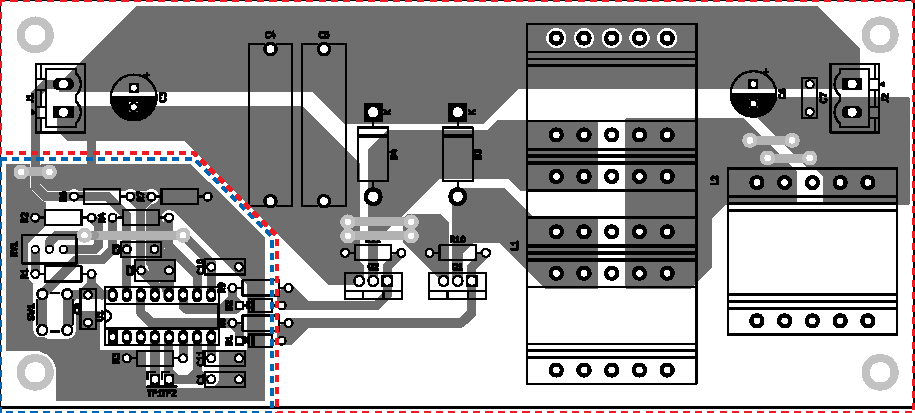
\includegraphics[scale=1]{pdf/layout/layout_CBI4.pdf}
        \label{fig:layout_cbi}
     	\indentedfont[15.5cm]{Elaboração própria (2021)}
    \end{figure}
    
    No desenvolvimento do \textit{layout}, teve-se o cuidado para isolar as referências de comando (azul) e potência (vermelho), como mostrado na \autoref{fig:layout_cbi}, e manter o fluxo de potência em um mesmo sentido, com laços de alta frequência pequenos, como pode ser observado na \autoref{fig:layout_cbi_boas_prat}.
    
    \begin{figure}[H]
    	\centering
    	\caption{Análise do \textit{layout} desenvolvido do CBI de dois ramos}
    	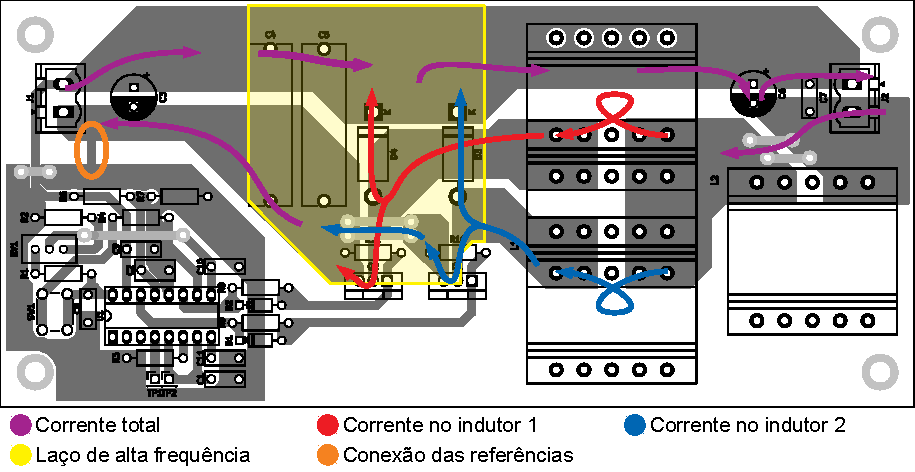
\includegraphics[scale=1]{pdf/layout/layout_CBI3.pdf}
        \label{fig:layout_cbi_boas_prat}
     	\indentedfont[15.5cm]{Elaboração própria (2021)}
    \end{figure}
    
    Finalizada a PCB, se iniciou os testes elétricos do CBI de dois ramos, para que fosse possível a validação do seu correto funcionamento. Nesses testes, foi percebido que, devido à elevada variação da corrente de saída, de aproximadamente \SI{2}{\ampere}, segundo \citeonline{ref:esr_capacitor}, o capacitor utilizado necessitaria de uma ESR máxima de \SI{6}{\milli$\Omega$}, para que assim fosse possível atender as especificações da variação de tensão de saída. Dessa forma, pela disponibilidade e dificuldade para se obter capacitores com ESR tão baixa, foi utilizado em paralelo dois capacitores eletrolítico de baixa resistência série, com valor de capacitância de \SI{470}{\micro\farad}. Assim, a \autoref{fig:esquematico_cbi_1} apresenta, sem o circuito de acionamento, o circuito de potência do conversor utilizado. 
    
    \begin{figure}[H]
    	\centering
    	\caption{Esquemático simplificado utilizado do CBI de dois ramos}
    	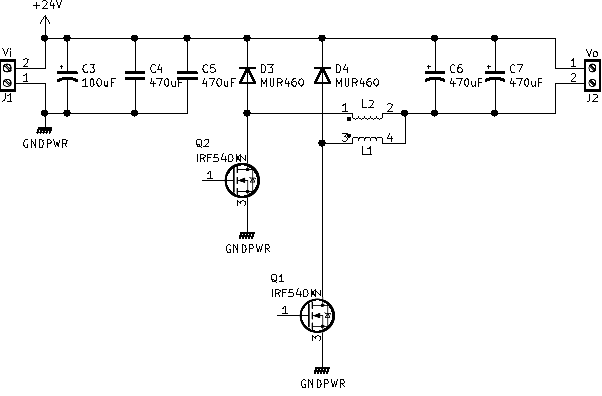
\includegraphics[scale=1.2]{pdf/layout/Esquematico_CBI_simples.pdf}
        \label{fig:esquematico_cbi_1}
     	\indentedfont[12.5cm]{Elaboração própria (2021)}
    \end{figure}
    
    O modelo 3D da placa desenvolvida para o conversor proposto pode ser observado na \autoref{fig:3d_placa_inicial}.
    
    \begin{figure}[H]
    	\centering
    	\caption{Modelo 3D do conversor desenvolvido}
    	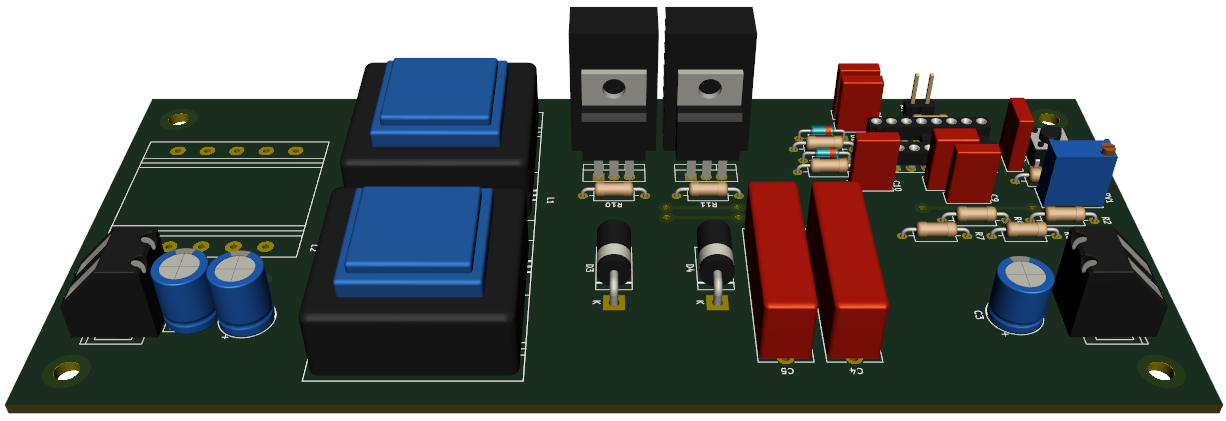
\includegraphics[scale=.35]{pdf/fotos/placa_inicial.png}
        \label{fig:3d_placa_inicial}
     	\indentedfont[15.5cm]{Elaboração própria (2021)}
    \end{figure}
    
    Após essas alterações, com exceção da variação da tensão de saída que permaneceu em \SI{2}{\%}, todos os demais requisitos elétricos estabelecidos para o projeto puderam ser alcançados e validados. Devido à especificação da variação da tensão de saída ser muita pequena, optou-se por mantê-la em \SI{2}{\%}, ao invés de aumentar a capacitância de saída.
    
    %%%%%%%%%%%%%%%%%%%%%%%%%%%%%%%%%%%%%%%%%%%%%%%%%%%%%%%%%%%%%%%%%%%
    \section{Padronização de medidas} \label{cap:result_padrao}
    %%%%%%%%%%%%%%%%%%%%%%%%%%%%%%%%%%%%%%%%%%%%%%%%%%%%%%%%%%%%%%%%%%%
    
    Após a validação elétrica do CBI de dois ramos, para que fosse possível realizar as medidas de EMI de forma mais confiável, sem impactos nos resultados provenientes de fatores alheios as técnicas propostas, foram feitas medições para averiguar a necessidade da padronização da medida.  
    
    A primeira medida realizada foi com relação a influência da posição do cabo na medida de EMI irradiada. Nesse teste, o cabo de alimentação e da carga do produto sob teste (o CBI de dois ramos) foram posicionados de duas formas distintas, cabo descendo de forma paralela até o chão da câmara (Medida 1) e cabo descendo de forma descuidada até o chão da câmara (Medida 2). A \autoref{fig:med_rad_cabo} apresenta os resultados obtidos com a medida. 
    
    \begin{figure}[H]
    	\centering
    	\caption{Espectro de emissão irradiada para o ensaio da influência do posicionamento do cabo de carga e alimentação nas medidas}
    	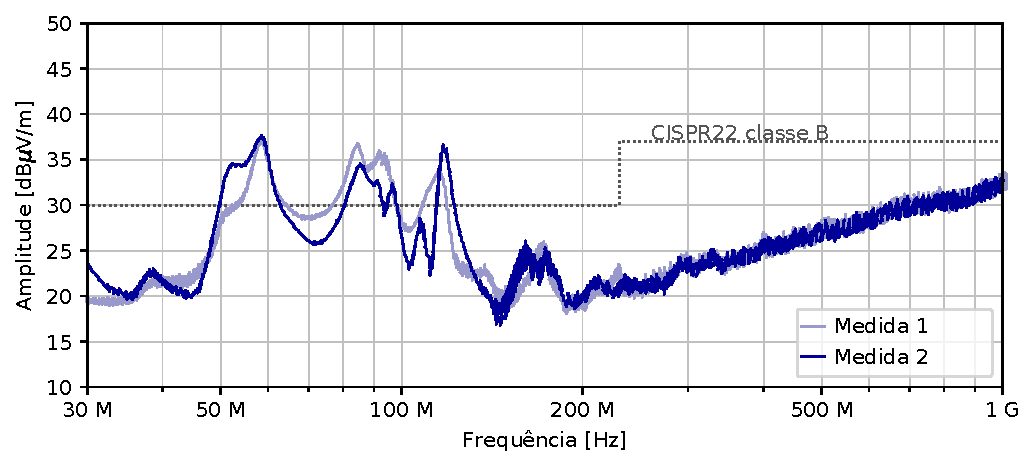
\includegraphics[scale=.9]{pdf/rad/Sem o cuidado com o cabo2.pdf}
    	\label{fig:med_rad_cabo}
     	\indentedfont[15.5cm]{Elaboração própria (2021)}
    \end{figure}
    
    Nota-se pela figura que o posicionamento dos cabos é de grande influência nas medidas. Dessa forma, evitando erros de medida, padronizou-se a posição do cabo como a utilizada na Medida 1.
    
    O segundo teste realizado foi do produto em regime térmico. Esse teste teve como objetivo verificar se haveria uma alteração na medida de EMI conduzida e irradiada do produto em temperatura ambiente e em regime térmico. Porém, após realizado, verificou-se que não havia variações nas medidas, podendo dessa forma realizar os testes futuros sem que houvesse a necessidade de deixar o produto em regime térmico antes de realizar as medidas. 
    
    Por último, após alguns testes, verificou-se a influência da rotação da placa dentro da câmara para um mesmo eixo medido nos testes de EMI irradiada. Nesse teste, percebeu-se que há uma grande variação na medida se os componentes presentes na placa estão voltados para a parede da câmara contendo o absorvedor de ondas electromagnéticas ou a porta da câmara. A \autoref{fig:med_rad_rot_placa} apresenta as medidas obtidas nesse teste para um dos eixos.
    
    \begin{figure}[H]
    	\centering
    	\caption{Espectro de emissão irradiada para o ensaio da rotação da placa dentro da câmara para um mesmo eixo}
    	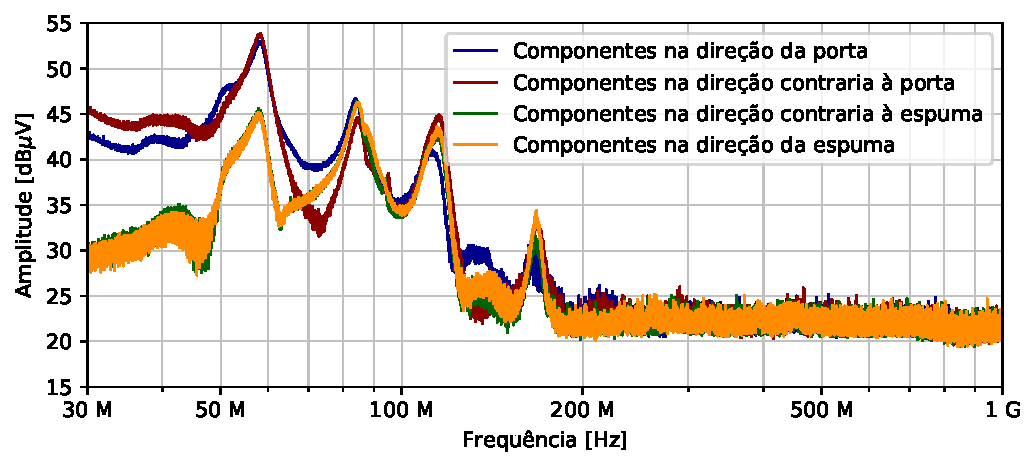
\includegraphics[scale=.9]{pdf/rad/rotacionando.pdf}
    	\label{fig:med_rad_rot_placa}
     	\indentedfont[15.5cm]{Elaboração própria (2021)}
    \end{figure}
    
    Com esse resultado, usou-se como padrão as medidas da placa com a face contendo os componentes voltada para a porta da câmara devido à maior facilidade de posicionamento.
    
    %%%%%%%%%%%%%%%%%%%%%%%%%%%%%%%%%%%%%%%%%%%%%%%%%%%%%%%%%%%%%%%%%%%
    \section{Técnicas de mitigação de EMI} \label{cap:result_tecnicas}
    %%%%%%%%%%%%%%%%%%%%%%%%%%%%%%%%%%%%%%%%%%%%%%%%%%%%%%%%%%%%%%%%%%%
    
    Tendo estabelecido um padrão de medida, pôde-se dar inicio aos testes de emissão conduzida e irradiada. Todos os testes realizados utilizaram como padrão comparativo a medida inicial (do CBI de dois ramos), para que seja possível analisar apenas os impactos gerados pela nova técnica. A \autoref{fig:med_cond_circ_inic} apresenta a medida inicial de EMI conduzida do CBI de dois ramos. 
    
    \begin{figure}[H]
    	\centering
    	\caption{Ensaio de emissão conduzida do conversor Buck \Interleaved}
    	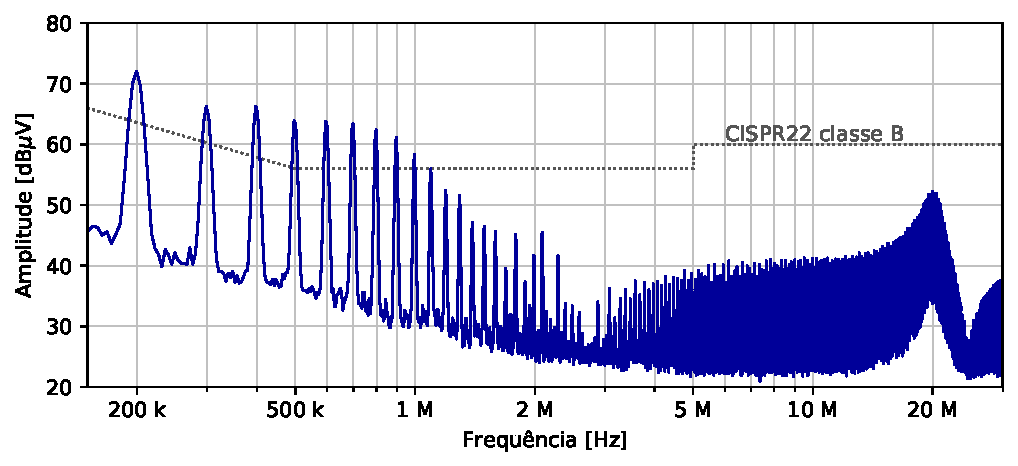
\includegraphics[scale=.9]{pdf/cond/Circuito inicial.pdf}
    	\label{fig:med_cond_circ_inic}
     	\indentedfont[15.5cm]{Elaboração própria (2021)}
    \end{figure}
    
    Nota-se pela figura que o conversor proposto apresenta elevados níveis de ruído conduzido em frequências múltiplas de \SI{100}{\kilo\hertz}. Tal fato se dá devido à haver no circuito dois chaveamentos em uma frequência de \SI{50}{\kilo\hertz} defasados em \SI{180}{\degree}. Ainda, destaca-se que há uma redução progressiva na amplitude dos harmônicos medidos, voltando a crescer após a frequência de \SI{3}{\mega\hertz}, com um pico em torno da frequência de \SI{20}{\mega\hertz}.
    
    Na \autoref{fig:med_rad_circ_inic} temos a medida inicial de EMI irradiada do CBI de dois ramos. 
    
    \begin{figure}[H]
    	\centering
    	\caption{Ensaio de emissão irradiada do conversor Buck \Interleaved}
    	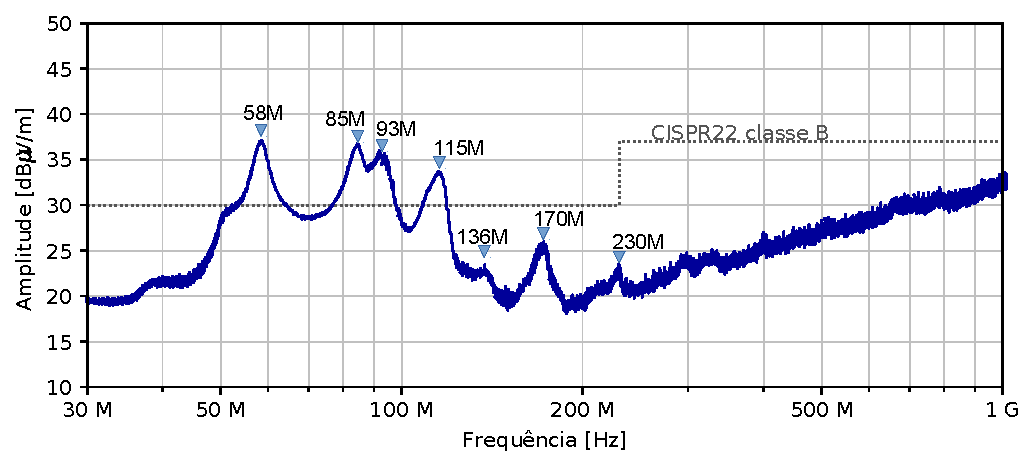
\includegraphics[scale=.9]{pdf/rad/Circuito inicial_2.pdf}
    	\label{fig:med_rad_circ_inic}
     	\indentedfont[15.5cm]{Elaboração própria (2021)}
    \end{figure}
    
    Nessa figura é possível observar alguns picos com amplitudes mais elevadas nas frequência do entorno de \SI{58}{\mega\hertz}, \SI{85}{\mega\hertz}, \SI{93}{\mega\hertz}, \SI{115}{\mega\hertz}, \SI{136}{\mega\hertz}, \SI{170}{\mega\hertz} e \SI{230}{\mega\hertz}, sendo esses picos de maior interesse de redução durante os testes das técnicas.
    
    Com as medidas obtidas, analisando o conversor proposto e a bibliografia, escolheu-se algumas técnicas de mitigação de EMI. As técnicas utilizadas foram apresentadas conforme o ponto de aplicação, sendo elas: o dissipador, o transistor, o indutor e a estrutura do conversor. 
    
    %%%%%%%%%%%%%%%%%%%%%%%%%%%%%%%%%%%%%%%%%%%%%%%%%%%%%%%%%%%%%%%%%%%
    \subsection{Técnicas relacionadas ao elemento dissipador} \label{cap:result_tecnicas_dissip}
    %%%%%%%%%%%%%%%%%%%%%%%%%%%%%%%%%%%%%%%%%%%%%%%%%%%%%%%%%%%%%%%%%%%
    
    A primeira técnica avaliada por esse trabalho, que visa analisar o impacto dos dissipadores nas medidas de emissão conduzida e irradiada, consiste na remoção dos dissipadores presentes nos transistores, representado na \autoref{fig:3d_tecnica_dissipador}. Tal teste foi possível devido aos transistores utilizados na estrutura, sem dissipador, quando em funcionamento, estarem dentro da faixa térmica limite de operação. 
    
    \begin{figure}[H]
    	\centering
    	\caption{Modelo 3D do conversor desenvolvido sem os dissipadores}
    	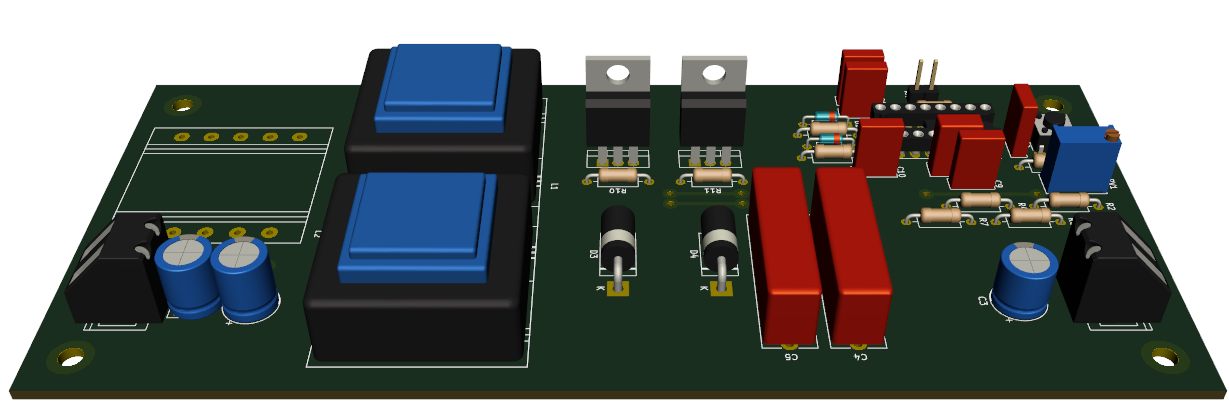
\includegraphics[scale=.35]{pdf/fotos/tecnica_dissipador.png}
        \label{fig:3d_tecnica_dissipador}
     	\indentedfont[15.5cm]{Elaboração própria (2021)}
    \end{figure}
    
    A \autoref{fig:med_cond_remv_dissip} apresenta um comparativo da emissão conduzida entre os resultados obtidos ao ser removido os dissipadores conectados aos transistores e a medida de referência (com os dissipadores conectados aos transistores). 
    
    \begin{figure}[H]
    	\centering
    	\caption{Comparação dos resultados do ensaio de emissão conduzida para o circuito sem os dissipadores e com os dissipadores conectados aos transistores}
    	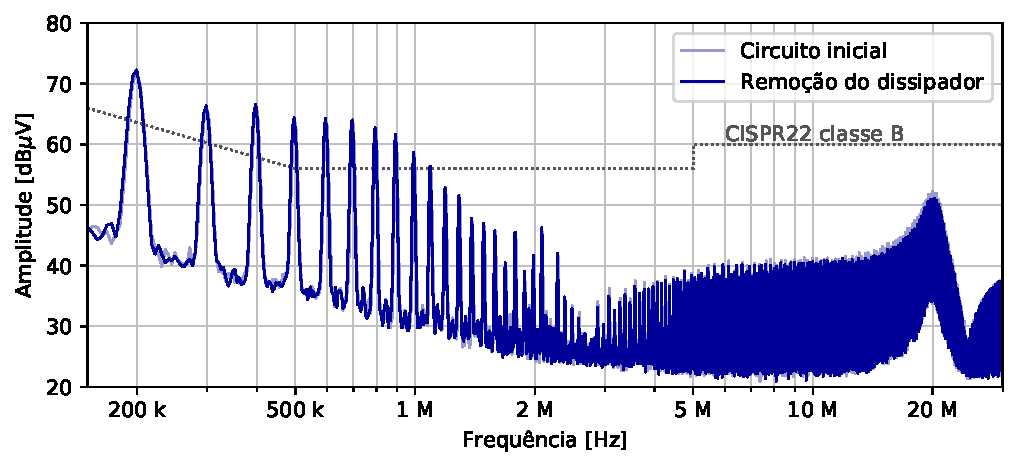
\includegraphics[scale=.9]{pdf/cond/Remoção do dissipador.pdf}
    	\label{fig:med_cond_remv_dissip}
     	\indentedfont[15.5cm]{Elaboração própria (2021)}
    \end{figure}
    
    Nota-se pela figura que não houve grandes mudanças nos resultados da emissão conduzida ao serem removidos os dissipadores, como já esperado, devido aos seus impactos serem principalmente na emissão irradiada. Dessa forma, a \autoref{fig:med_rad_remv_dissip} apresenta o comparativo da emissão irradiada entre os resultados obtidos ao serem removidos os dissipadores conectados aos transistores e a medida de referência. 
    
    \begin{figure}[H]
    	\centering
    	\caption{Comparação dos resultados do ensaio de emissão irradiada para o circuito sem os dissipadores e com os dissipadores conectados aos transistores}
    	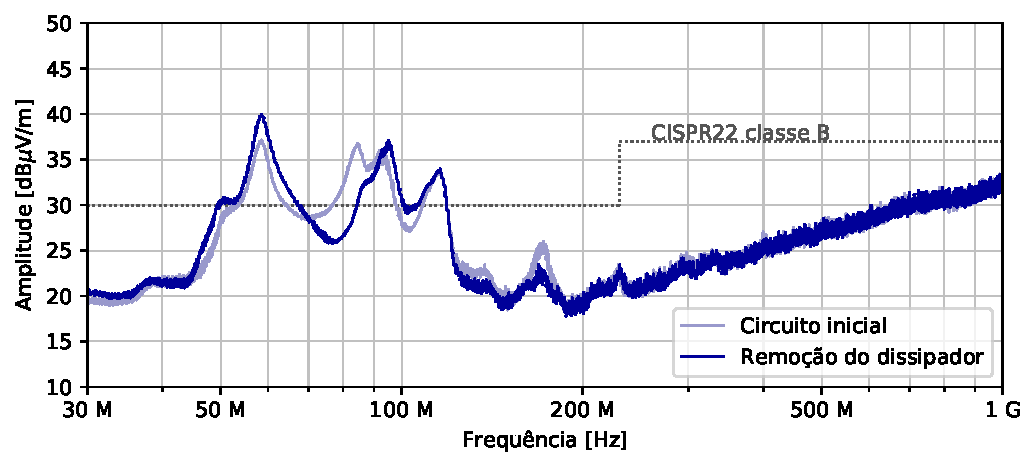
\includegraphics[scale=.9]{pdf/rad/Remoção do dissipador.pdf}
    	\label{fig:med_rad_remv_dissip}
     	\indentedfont[15.5cm]{Elaboração própria (2021)}
    \end{figure}
    
    Pela figura, percebe-se uma pequena alteração dos resultados obtidos. No entorno das frequências de \SI{58}{\mega\hertz} e \SI{93}{\mega\hertz} houve um pequeno acréscimo na emissão irradiada, enquanto nas frequências de \SI{85}{\mega\hertz} e \SI{170}{\mega\hertz} se obteve uma redução. Dessa forma, essa técnica não apresentou grandes benefícios para a redução das emissões. 
    
    Outra medida realizada, relacionada aos dissipadores, foi a conexão do dissipador a referência utilizando um capacitor cerâmico $\subx{C}{D}$, conforme \autoref{fig:esquematico_cbi_2}. O capacitor foi necessário devido ao dissipador não estar isolado e, portanto, conectado diretamente ao dreno do transistor. Nesta técnica, busca-se criar um caminho de menor impedância para os harmônicos gerados, evitado que o mesmo seja irradiado pelo dissipador. 
    
    \begin{figure}[H]
    	\centering
    	\caption{Esquemático simplificado do CBI de dois ramos com a conexão do dissipador a referência do circuito}
    	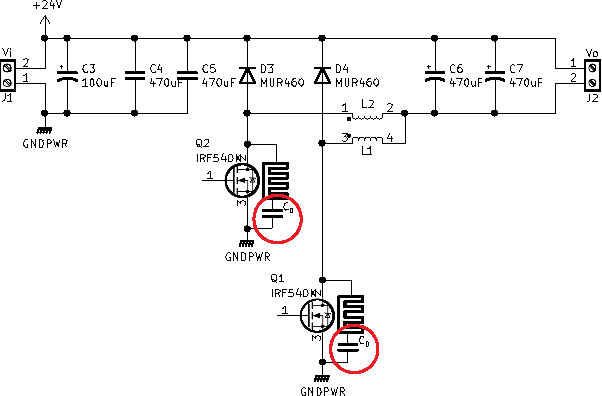
\includegraphics[scale=1.2]{pdf/layout/Esquematico_CBI_dissipador2.pdf}
        \label{fig:esquematico_cbi_2}
     	\indentedfont[12.5cm]{Elaboração própria (2021)}
    \end{figure}
    
    
    O modelo 3D da técnica aplicada no conversor pode ser observada na \autoref{fig:3d_tecnica_capacitor}.
    
    \begin{figure}[H]
    	\centering
    	\caption{Modelo 3D do conversor desenvolvido com capacitores conectados aos dissipadores}
    	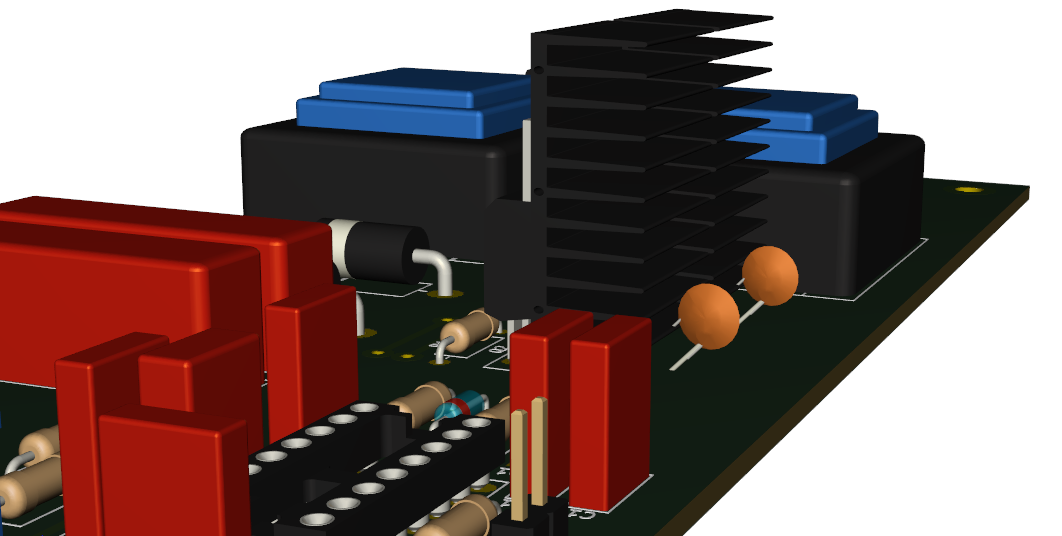
\includegraphics[scale=.35]{pdf/fotos/tecnica_capacitor.png}
        \label{fig:3d_tecnica_capacitor}
     	\indentedfont[15.5cm]{Elaboração própria (2021)}
    \end{figure}
    
    Para esse ensaio, foram arbitrados dois capacitores de diferentes valores, \SI{1}{\nano\farad} e \SI{100}{\nano\farad}, para que fosse possível verificar os impactos gerados pelos valores escolhidos. A \autoref{fig:med_cond_cap1n_dissip} apresenta um comparativo dos resultados obtidos do ensaio de emissão conduzida para o circuito com os dissipadores desconectados e conectados à referência via capacitor de \SI{1}{\nano\farad}.
    
    \begin{figure}[H]
    	\centering
    	\caption{Comparação dos resultados do ensaio de emissão conduzida para o circuito com os dissipadores desconectados e conectados à referência via capacitor de \SI{1}{\nano\farad}}
    	\includegraphics[scale=.9]{pdf/cond/Conectar o dissipador a referência (Capacitor de 1nF).pdf}
    	\label{fig:med_cond_cap1n_dissip}
     	\indentedfont[15.5cm]{Elaboração própria (2021)}
    \end{figure}
    
    Percebe-se que o uso do capacitor, diferentemente da remoção dos dissipadores, impactou na emissão conduzida do ruído. É possível observar na medida que, após a alteração, os harmônicos múltiplos de \SI{50}{\kilo\hertz} estão com maior amplitude do que na medida inicial. Ainda, no entorno da frequência de \SI{20}{\mega\hertz} é perceptível um aumento ainda mais acentuado dos harmônicos. 
    
    A medida de emissão irradiada desse teste, para o circuito com os dissipadores conectados à referência via capacitor de \SI{1}{\nano\farad}, pode ser observado na \autoref{fig:med_rad_cap1n_dissip}. 
    
    \begin{figure}[H]
    	\centering
    	\caption{Comparação dos resultados do ensaio de emissão irradiada para o circuito com os dissipadores desconectados e conectados à referência via capacitor de \SI{1}{\nano\farad}}
    	\includegraphics[scale=.9]{pdf/rad/Conectar o dissipador a referência (Capacitor de 1nF).pdf}
    	\label{fig:med_rad_cap1n_dissip}
     	\indentedfont[15.5cm]{Elaboração própria (2021)}
    \end{figure}
    
    Nessa figura, observa-se que houve grandes reduções em dois principais picos da emissão irradiada nas frequências de \SI{58}{\mega\hertz} e \SI{115}{\mega\hertz}. Ainda, destaca-se a redução de amplitude em frequências inferiores a \SI{70}{\mega\hertz}. Porém, têm-se uma elevação na amplitude em outras frequências. 
    
    Essa técnica, utilizando um capacitor de \SI{1}{\nano\farad}, apesar de apresentar melhoras em determinadas frequências na emissão irradiada, apresentou pioras em outras frequências, inclusive na emissão conduzida. A \autoref{fig:med_cond_cap100n_dissip} apresenta a mesma técnica, porém utilizando um capacitor de \SI{100}{\nano\farad}, para a emissão conduzida.
    
    \begin{figure}[H]
    	\centering
    	\caption{Comparação dos resultados do ensaio de emissão conduzida para o circuito com os dissipadores desconectados e conectados a referência via capacitor de \SI{100}{\nano\farad}}
    	\includegraphics[scale=.9]{pdf/cond/Conectar o dissipador a referência (Capacitor de 100nF).pdf}
    	\label{fig:med_cond_cap100n_dissip}
     	\indentedfont[15.5cm]{Elaboração própria (2021)}
    \end{figure}
    
    Nota-se que, diferente do resultado obtido para um capacitor de \SI{1}{\nano\farad}, ao utilizar um capacitor cerâmico de \SI{100}{\nano\farad}, há uma redução da amplitude da emissão conduzida no entorno da frequência de \SI{20}{\mega\hertz}. 
    
    O comparativo da emissão irradiada desse teste, para o circuito com os dissipadores conectados e desconectados da referência pode ser observado na \autoref{fig:med_rad_cap100n_dissip}.
    
    \begin{figure}[H]
    	\centering
    	\caption{Comparação dos resultados do ensaio de emissão irradiada para o circuito com os dissipadores desconectados e conectados a referência via capacitor de \SI{100}{\nano\farad}}
    	\includegraphics[scale=.9]{pdf/rad/Conectar o dissipador a referência (Capacitor de 100nF).pdf}
    	\label{fig:med_rad_cap100n_dissip}
     	\indentedfont[15.5cm]{Elaboração própria (2021)}
    \end{figure}
    
    Na figura, pode-se verificar que o uso de um capacitor de \SI{100}{\nano\farad} gerou uma grande redução nos níveis de emissão irradiada para quase todas as frequências, com exceção de poucas frequências, como o caso do entorno de \SI{170}{\mega\hertz}. Assim, percebe-se que, para o conversor proposto, o uso da técnica de aterramento do dissipador apresenta melhores resultados, se comparado a remoção do dissipador. Porém, a escolha do valor da capacitância é de grande impacto nos resultados, como pode-se observar na \autoref{fig:med_cond_cap1n_cap100n_dissip}, que apresenta o comparativos dos resultados obtidos da emissão conduzida.
    
    \begin{figure}[H]
    	\centering
    	\caption{Comparação dos resultados do ensaio de emissão conduzida para o circuito com os dissipadores conectados a referência via capacitor de \SI{1}{\nano\farad} e \SI{100}{\nano\farad}}
    	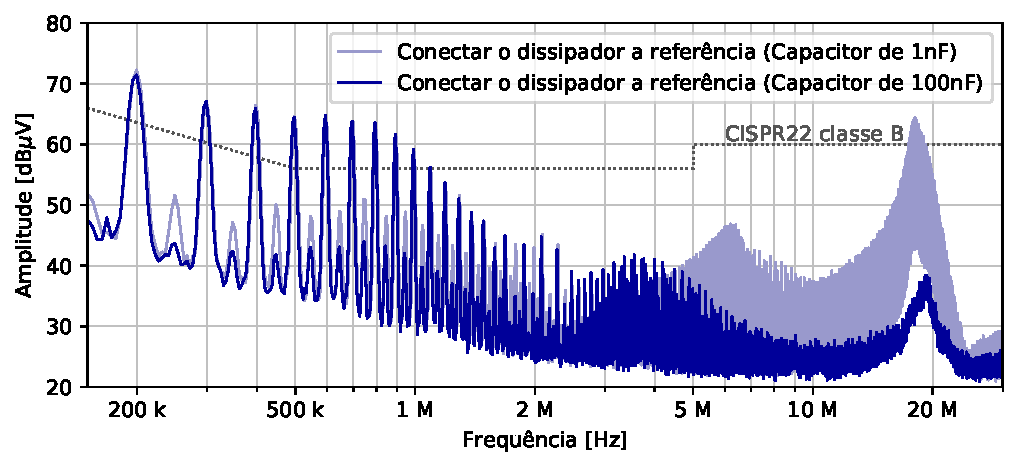
\includegraphics[scale=.85]{pdf/cond/cond-Conectar o dissipador a referência (Capacitor de 1nF)-Conectar o dissipador a referência (Capacitor de 100nF).pdf}
    	\label{fig:med_cond_cap1n_cap100n_dissip}
     	\indentedfont[15.5cm]{Elaboração própria (2021)}
    \end{figure}
    
    O mesmo comprativo, para a emissão irradiada, pode ser observada na \autoref{fig:med_rad_cap1n_cap100n_dissip}.
    
    \begin{figure}[H]
    	\centering
    	\caption{Comparação dos resultados do ensaio de emissão irradiada para o circuito com os dissipadores conectados a referência via capacitor de \SI{1}{\nano\farad} e \SI{100}{\nano\farad}}
    	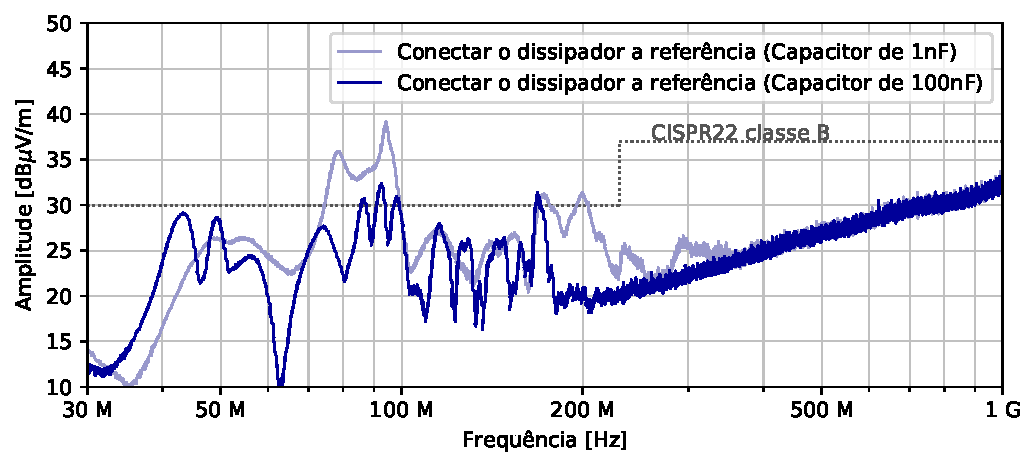
\includegraphics[scale=.85]{pdf/rad/Conectar o dissipador a referência (Capacitor de 1nF)-Conectar o dissipador a referência (Capacitor de 100nF).pdf}
    	\label{fig:med_rad_cap1n_cap100n_dissip}
     	\indentedfont[15.5cm]{Elaboração própria (2021)}
    \end{figure}

    %%%%%%%%%%%%%%%%%%%%%%%%%%%%%%%%%%%%%%%%%%%%%%%%%%%%%%%%%%%%%%%%%%%
    \subsection{Técnicas relacionadas ao elemento transistor} \label{cap:result_tecnicas_chaveam}
    %%%%%%%%%%%%%%%%%%%%%%%%%%%%%%%%%%%%%%%%%%%%%%%%%%%%%%%%%%%%%%%%%%%
    
    Outra técnica avaliada por esse trabalho, relacionada ao chaveamento do transistor, consiste no aumento do tempo de subida do sinal de dreno. Para esse teste, foi feita uma alteração nos resistores R8 e R9, conforme \autoref{fig:esquematico_cbi_3}, que possuíam valores iniciais de \SI{22}{$\Omega$} (com tempo de subida $\subx{t}{r}$ medido em osciloscópio de \SI{138}{\nano\second}) para um valor de \SI{62}{$\Omega$} (com tempo de subida $\subx{t}{r}$ medido em osciloscópio de \SI{255}{\nano\second}). 
    
    \begin{figure}[H]
    	\centering
    	\caption{Esquemático simplificado do CBI de dois ramos com a alteração nos valores dos resistores R8 e R9}
    	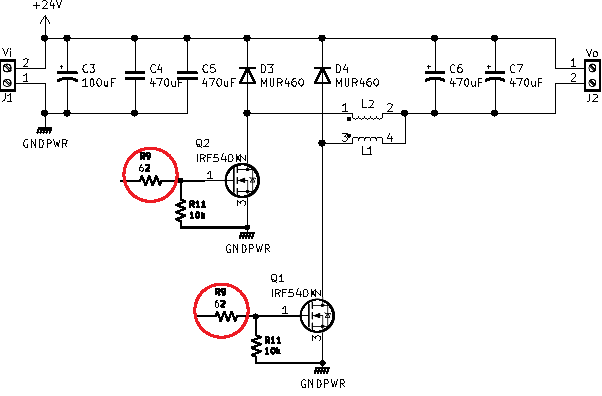
\includegraphics[scale=1.2]{pdf/layout/Esquematico_CBI_tr.pdf}
        \label{fig:esquematico_cbi_3}
     	\indentedfont[12.5cm]{Elaboração própria (2021)}
    \end{figure}
    
    Assim, a \autoref{fig:med_cond_temp_sub} apresenta um comparativo da emissão conduzida entre os resultados obtidos para o circuito inicial ($\subx{t}{r}$ de \SI{138}{\nano\second}) e circuito após alteração dos resistores ($\subx{t}{r}$ de \SI{255}{\nano\second}). 
    
    \begin{figure}[H]
    	\centering 
    	\caption{Comparação dos resultados do ensaio de emissão conduzida para um tempo de subida do sinal no dreno do transistor de \SI{138}{\nano\second} e \SI{255}{\nano\second}}
    	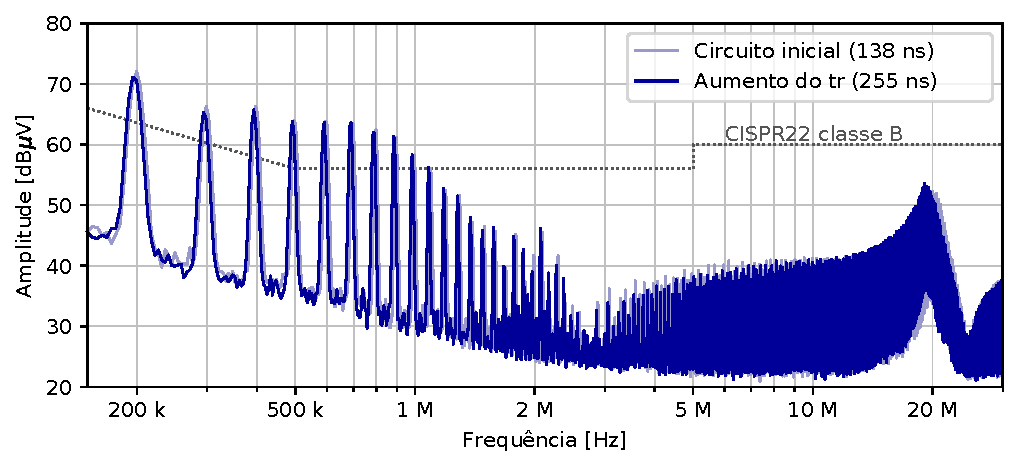
\includegraphics[scale=.9]{pdf/cond/Aumento do tr do transistor2.pdf}
    	\label{fig:med_cond_temp_sub}
     	\indentedfont[15.5cm]{Elaboração própria (2021)}
    \end{figure}
    
    Percebe-se pela figura que a alteração desse tempo de subida não acarretou em grandes alterações nas medidas de emissão conduzida. Na \autoref{fig:med_rad_temp_sub} é possível observar o comparativo da emissão irradiada para o mesmo teste.  
    
    \begin{figure}[H]
    	\centering
    	\caption{Comparação dos resultados do ensaio de emissão irradiada para um tempo de subida do sinal no dreno do transistor de \SI{138}{\nano\second} e \SI{255}{\nano\second}}
    	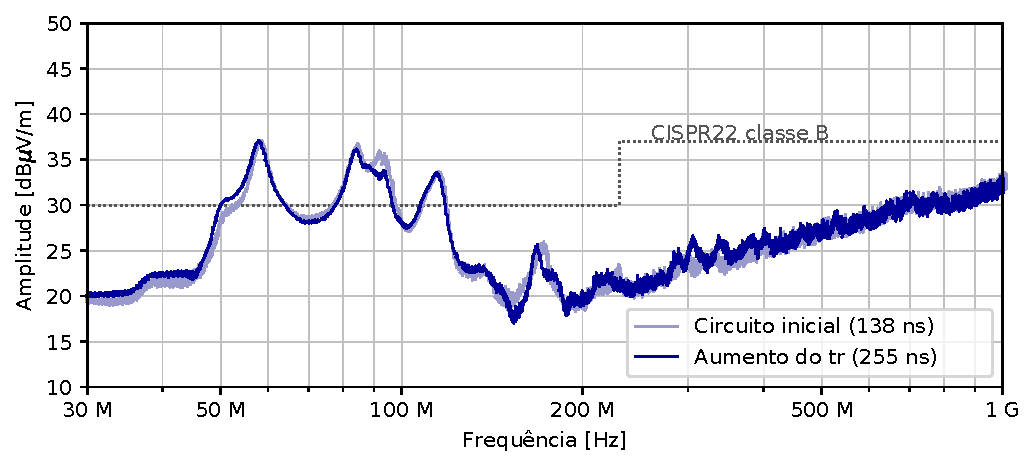
\includegraphics[scale=.9]{pdf/rad/Aumento do tr do transistor2.pdf}
    	\label{fig:med_rad_temp_sub}
     	\indentedfont[15.5cm]{Elaboração própria (2021)}
    \end{figure}
    
    Na emissão irradiada também não houve grandes impactos gerados pela técnica. Esse resultado é devido ao tempo de subida no dreno já ser grande (proveniente do resistor de \SI{22}{$\Omega$}) e assim, esse aumento no tempo de subida, não surtiu efeito para as emissões. 
    
    Ainda relacionado ao dreno do transistor, outra técnica empregada no circuito foi o uso de um núcleo de ferrite \textit{bead} nos terminais de dreno do transistor, como mostrado na \autoref{fig:esquematico_cbi_4}. 
    
    \begin{figure}[H]
    	\centering
    	\caption{Esquemático simplificado do CBI de dois ramos com um núcleo de ferrite no terminal de dreno dos transistores}
    	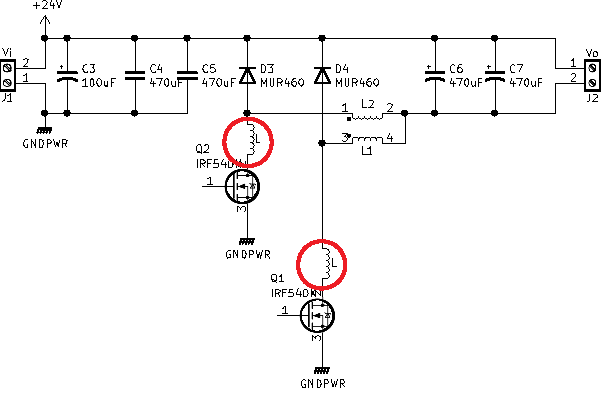
\includegraphics[scale=1.2]{pdf/layout/Esquematico_CBI_bead.pdf}
        \label{fig:esquematico_cbi_4}
     	\indentedfont[12.5cm]{Elaboração própria (2021)}
    \end{figure}
    
    A \autoref{fig:3d_tecnica_choke} apresenta um modelo 3D da técnica aplicada ao conversor.
    
    \begin{figure}[H]
    	\centering
    	\caption{Modelo 3D do conversor desenvolvido com um núcleo de ferrite no terminal de dreno dos transistores}
    	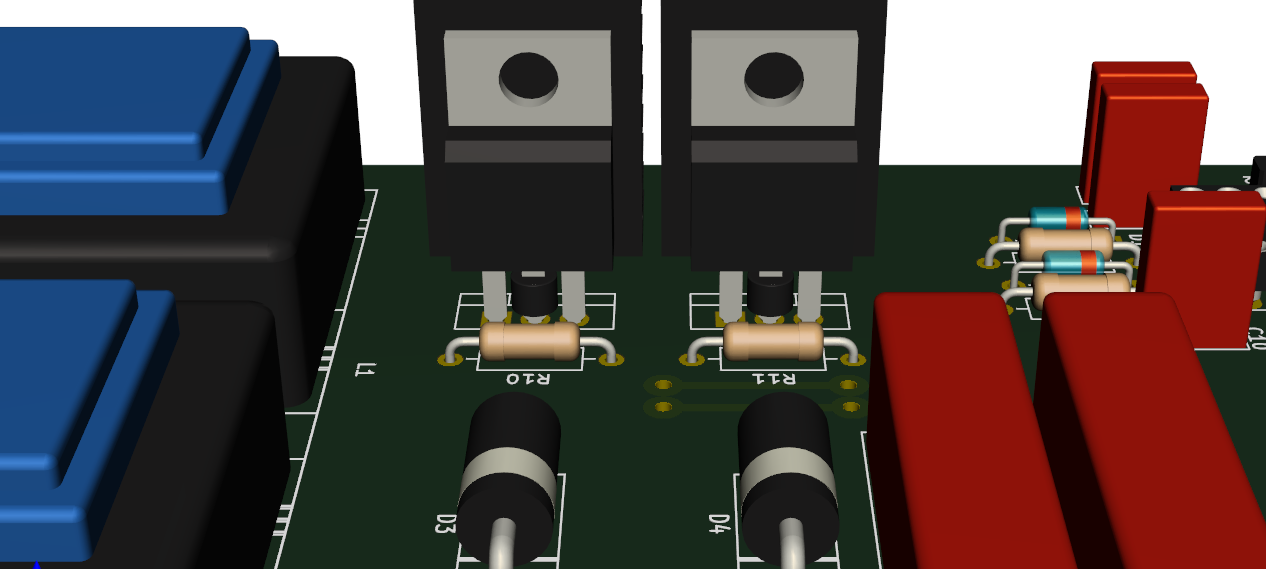
\includegraphics[scale=.35]{pdf/fotos/tecnica_choke2.png}
        \label{fig:3d_tecnica_choke}
     	\indentedfont[15.5cm]{Elaboração própria (2021)}
    \end{figure}
    
    Esta técnica busca confinar no transistor os harmônicos gerados por ele. A \autoref{fig:med_cond_choke} apresenta o comparativo da emissão conduzida entre os resultados obtidos para o circuito inicial (sem o núcleo de ferrite) e o circuito após inserção do núcleo de ferrite \textit{bead}. 
    
    \begin{figure}[H]
    	\centering 
    	\caption{Comparação dos resultados do ensaio de emissão conduzida para o circuito com e sem um núcleo de ferrite nos terminais de dreno dos transistores}
    	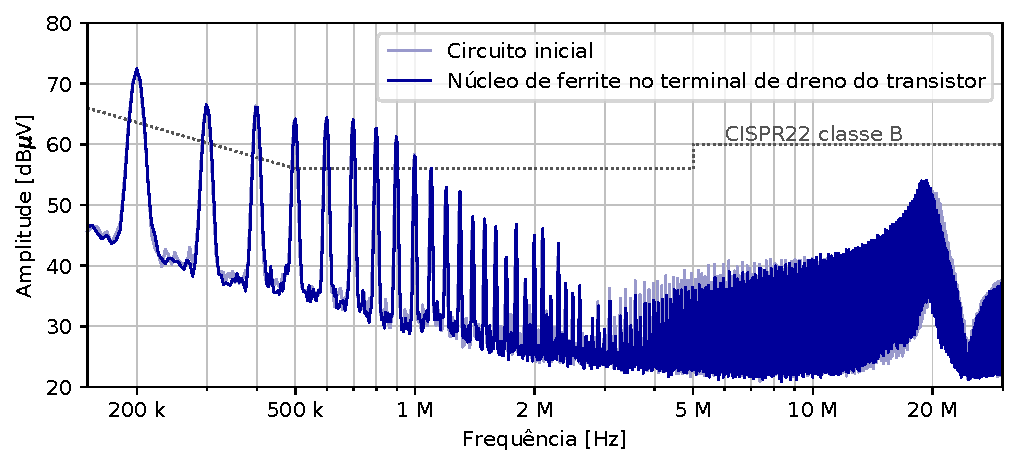
\includegraphics[scale=.9]{pdf/cond/Choke bead no terminal de dreno do transistor.pdf}
    	\label{fig:med_cond_choke}
     	\indentedfont[15.5cm]{Elaboração própria (2021)}
    \end{figure}
    
    Nessa técnica, para a emissão conduzida, também não houve grandes alterações nos resultados. Porém, para a emissão irradiada, algumas mudanças podem ser observadas nas medidas, como na \autoref{fig:med_rad_temp_sub}.  
    
    \begin{figure}[H]
    	\centering
    	\caption{Comparação dos resultados do ensaio de emissão irradiada para o circuito com e sem um núcleo de ferrite nos terminais de dreno dos transistores}
    	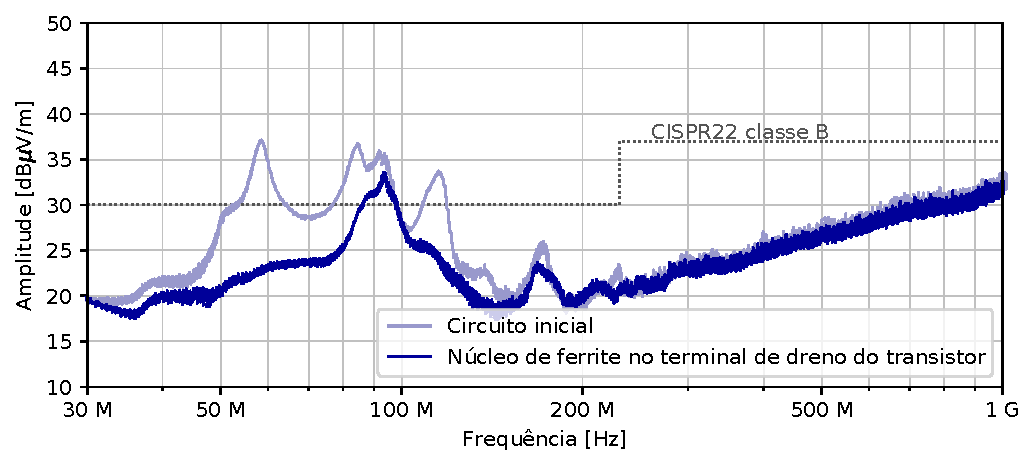
\includegraphics[scale=.9]{pdf/rad/Choke bead no terminal de dreno do transistor.pdf}
    	\label{fig:med_rad_choke}
     	\indentedfont[15.5cm]{Elaboração própria (2021)}
    \end{figure}
    
    Essa técnica mostrou grande eficácia na redução do ruído irradiado, ao contrário da emissão conduzida. Como pode-se observar, a técnica apresentou redução em uma larga faixa de frequência (entre \SI{30}{\mega\hertz} e \SI{200}{\mega\hertz}), com apenas dois picos próximos dos valores iniciais medidos (\SI{93}{\mega\hertz} e \SI{170}{\mega\hertz}).
    
    %%%%%%%%%%%%%%%%%%%%%%%%%%%%%%%%%%%%%%%%%%%%%%%%%%%%%%%%%%%%%%%%%%%
    \subsection{Técnica relacionada ao elemento indutor} \label{cap:result_tecnicas_indut}
    %%%%%%%%%%%%%%%%%%%%%%%%%%%%%%%%%%%%%%%%%%%%%%%%%%%%%%%%%%%%%%%%%%%
    
    Com relação aos indutores, buscando reduzir o acoplamento entre eles, utilizou-se como técnica o reposicionamento de um deles, o rotacionando. Na \autoref{fig:foto_cbi_1} é possível observar a placa inicialmente produzida, com os indutores circulados em vermelho. 
    
    \begin{figure}[H]
    	\centering
    	\caption{Posicionamento dos indutores no circuito inicial}
    	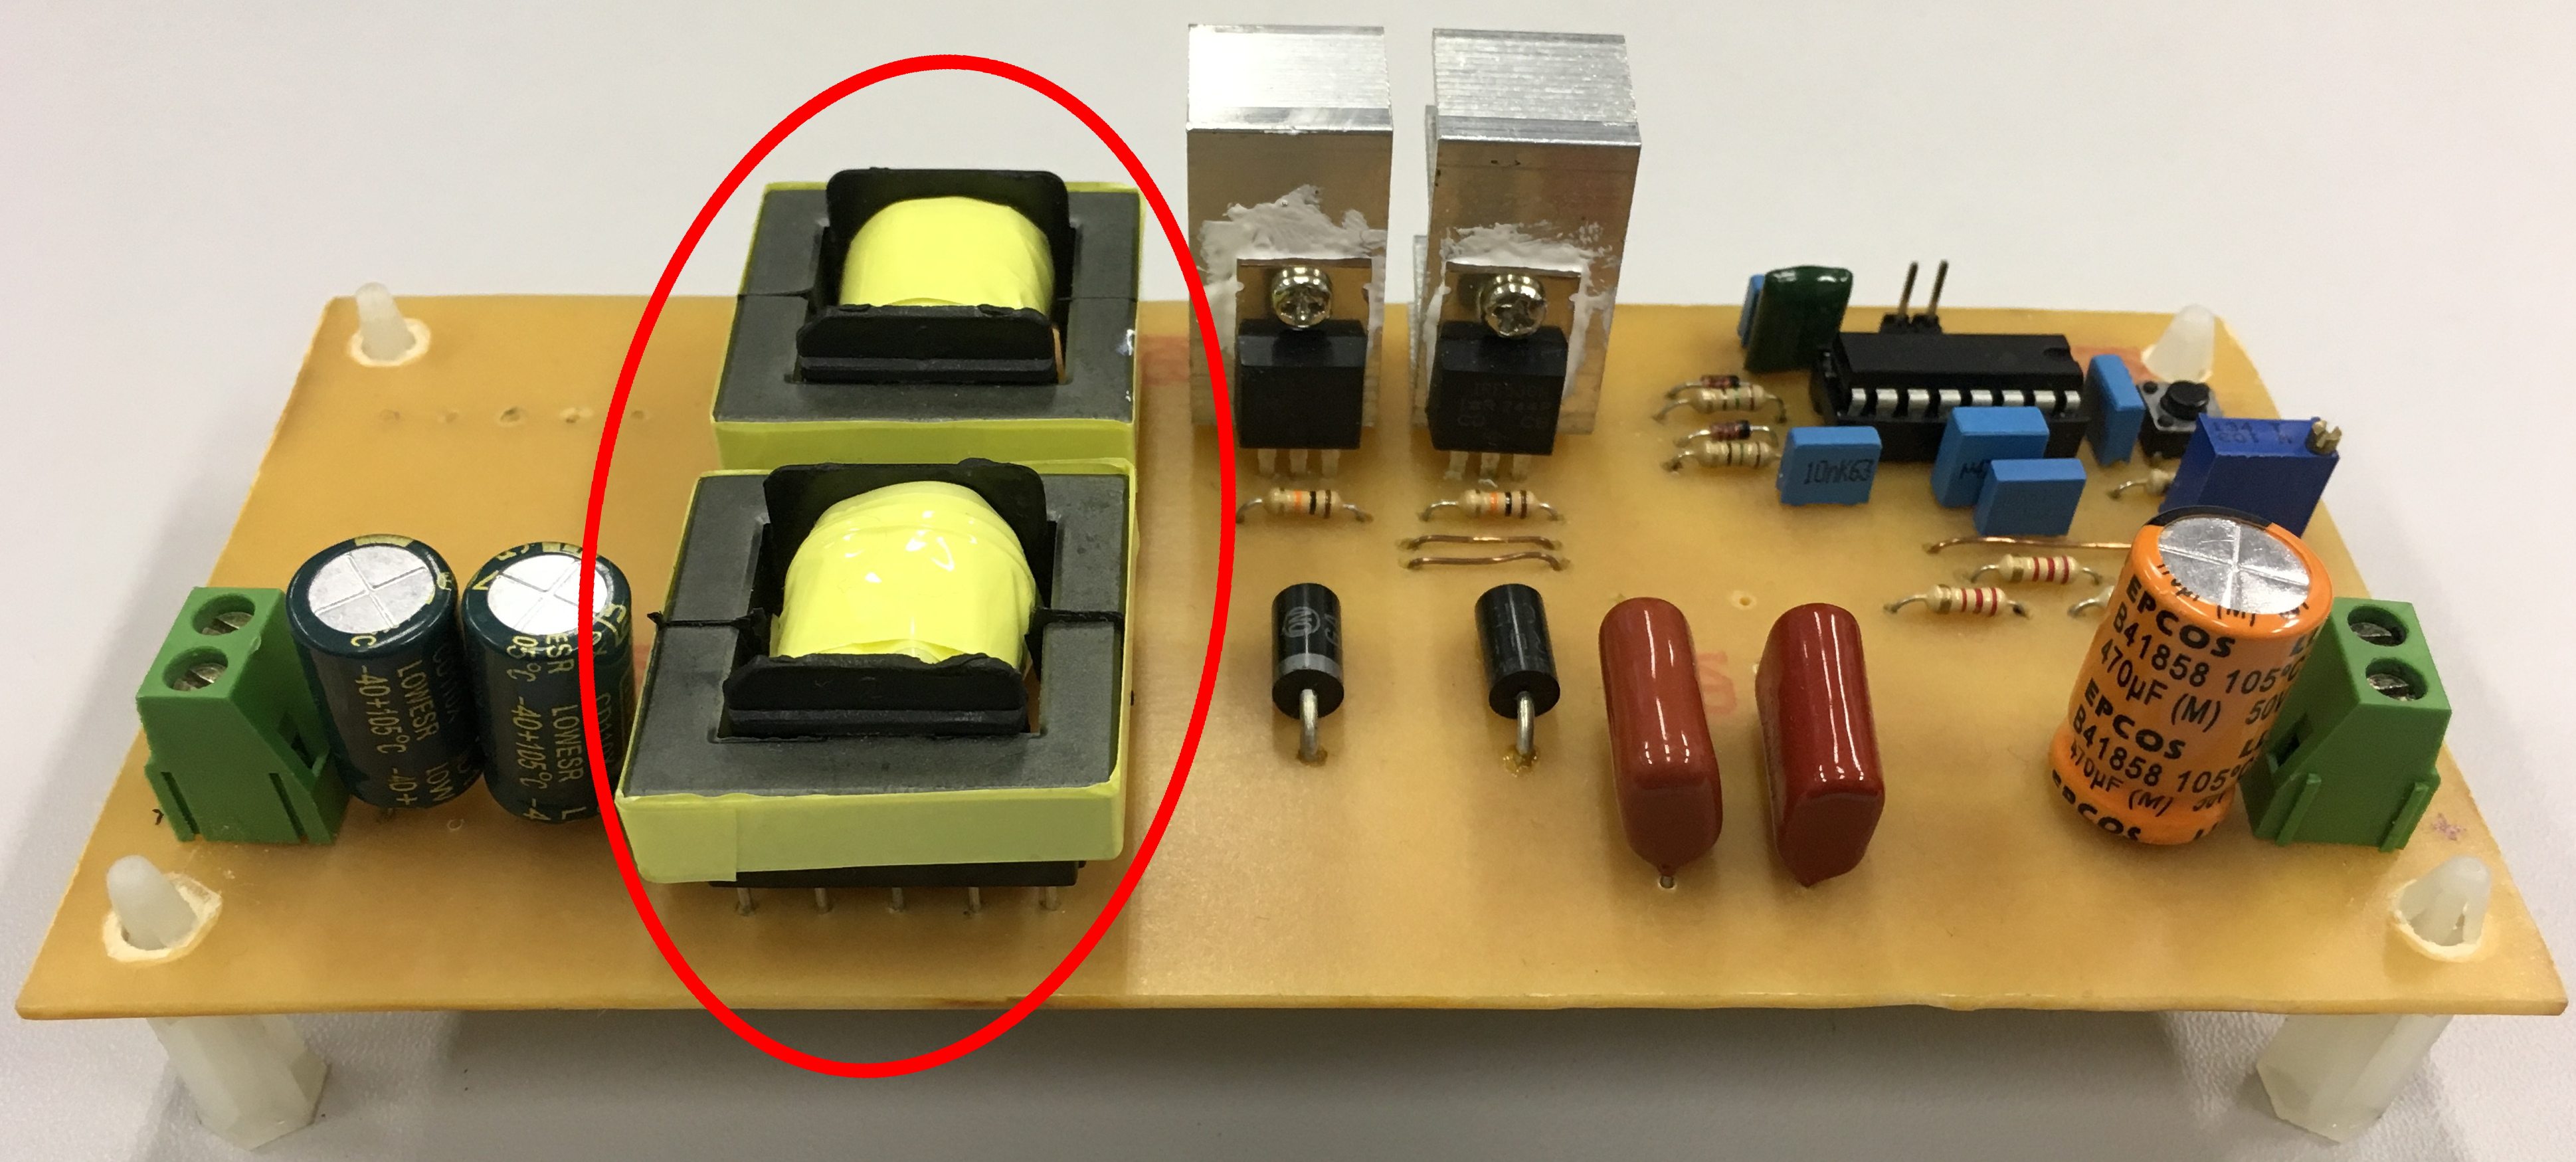
\includegraphics[scale=.1]{pdf/fotos/placa_vista_lateral_sel.jpg}
        \label{fig:foto_cbi_1}
     	\indentedfont[14cm]{Elaboração própria (2021)}
    \end{figure}
    
    Percebe-se pela figura, que ambos os indutores estão posicionados paralelamente e com seus fluxos na mesma direção, como demonstrado na \autoref{fig:foto_cbi_2}.
    
    \begin{figure}[H]
    	\centering
    	\caption{Representação do fluxo dos indutores no circuito inicial}
    	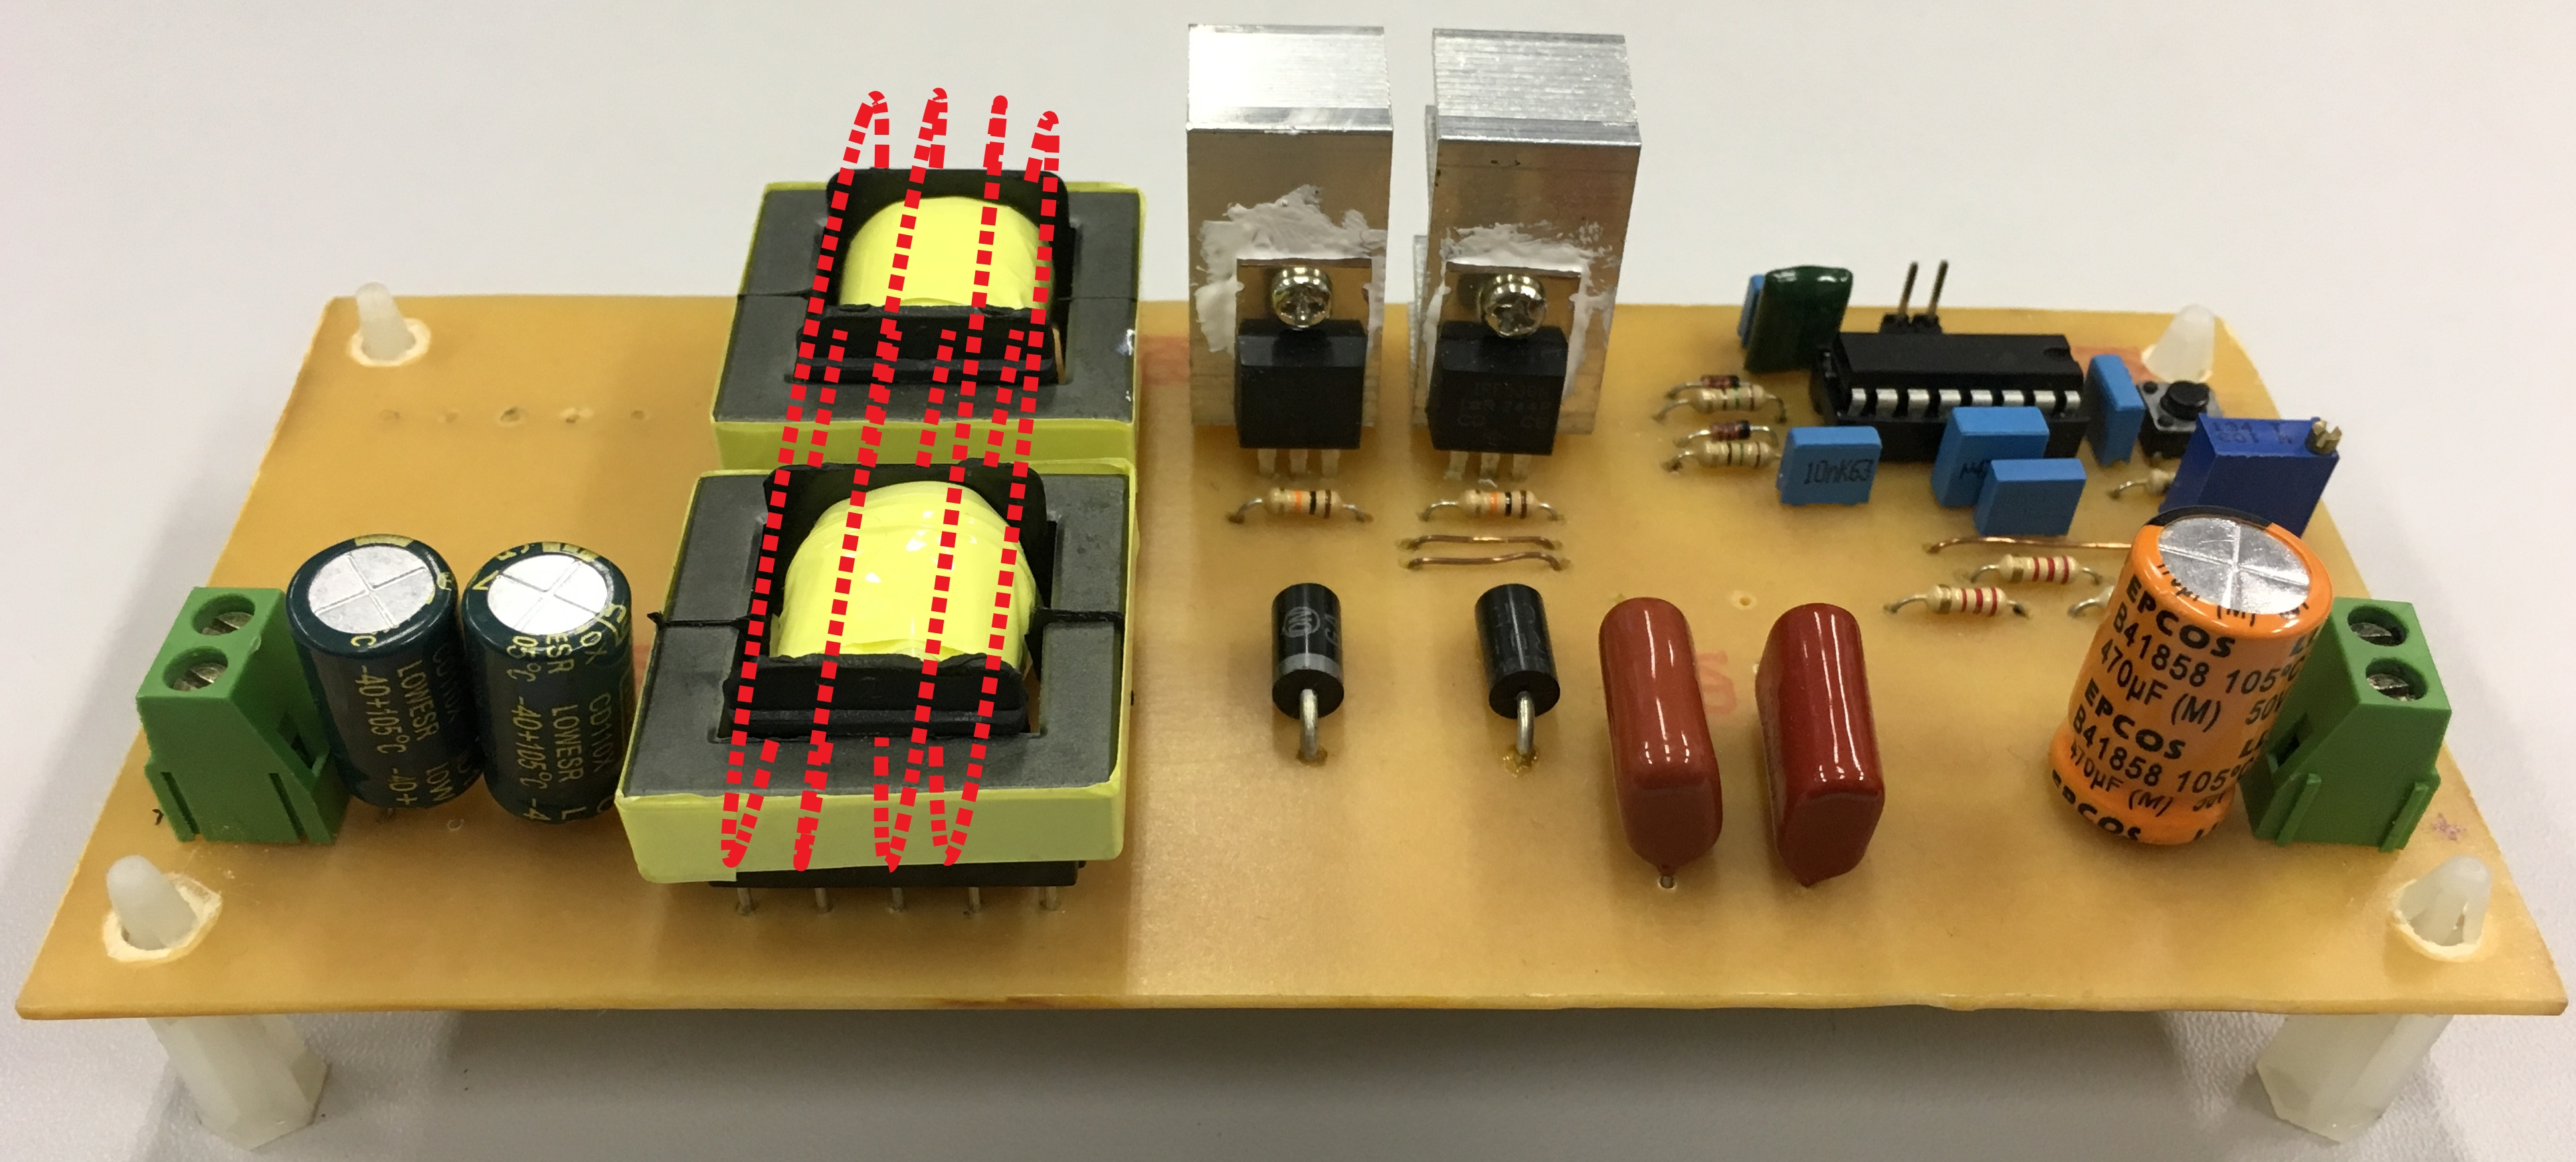
\includegraphics[scale=.1]{pdf/fotos/placa_vista_lateral_fluxo.jpg}
        \label{fig:foto_cbi_2}
     	\indentedfont[14cm]{Elaboração própria (2021)}
    \end{figure}
    
    Dessa forma, a mudança de posição de um dos indutores, como na \autoref{fig:foto_cbi_3}, proporciona uma mudança na direção do fluxo magnético disperso no ar, gerando um menor acoplamento entre ambos. 
    %um dos indutores presentes foi rotacionado, como mostra a \autoref{fig:foto_cbi_3}, buscando um menor acoplamento entre ambos. 
    
    \begin{figure}[H]
    	\centering
    	\caption{Representação da placa com um indutor rotacionado indutores no circuito inicial}
    	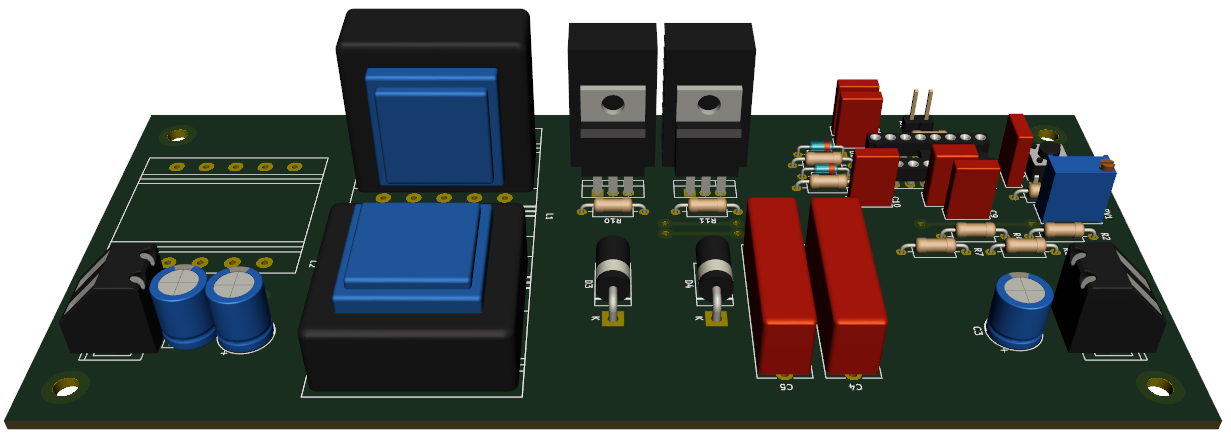
\includegraphics[scale=.3]{pdf/fotos/tecnica_indutor.png}
        \label{fig:foto_cbi_3}
     	\indentedfont[14cm]{Elaboração própria (2021)}
    \end{figure}
    
    O  comparativo da emissão conduzida entre os resultados obtidos para o circuito inicial e após o reposicionamento do indutor, pode ser observado na \autoref{fig:med_cond_indutor}.
    
    \begin{figure}[H]
    	\centering
    	\caption{Comparação dos resultados do ensaio de emissão conduzida para o circuito inicial e com um dos indutores rotacionado}
    	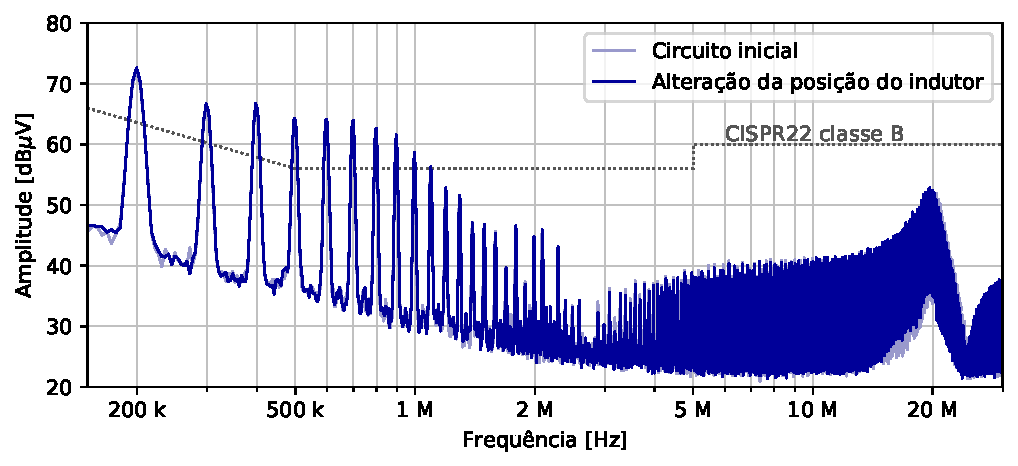
\includegraphics[scale=.9]{pdf/cond/Alteração da posição do indutor.pdf}
    	\label{fig:med_cond_indutor}
     	\indentedfont[15.5cm]{Elaboração própria (2021)}
    \end{figure}
    
    Observa-se que para a emissão conduzida não houve mudanças nos resultados. Na \autoref{fig:med_rad_indutor}, tem-se os resultados obtidos para a mesma técnica para a emissão irradiada. 
    
    \begin{figure}[H]
    	\centering
    	\caption{Comparação dos resultados do ensaio de emissão irradiada para o circuito inicial e com um dos indutores rotacionado}
    	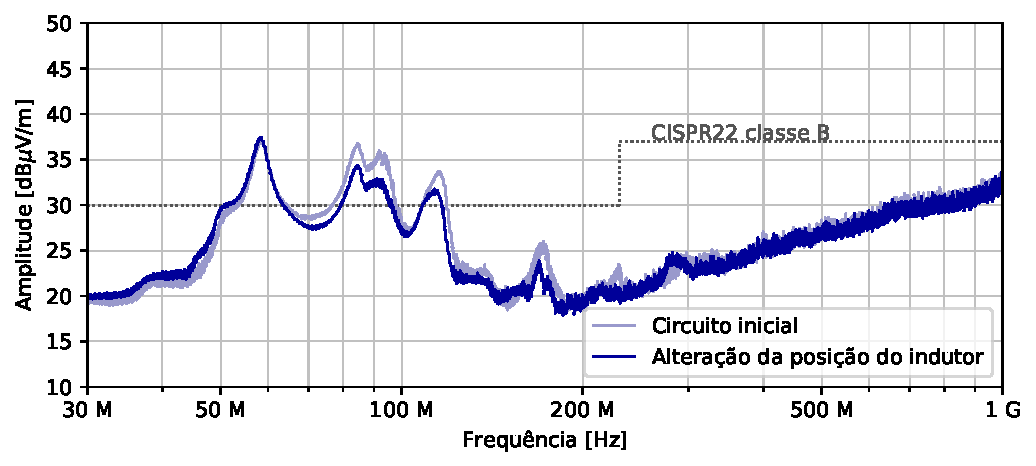
\includegraphics[scale=.9]{pdf/rad/Alteração da posição do indutor.pdf}
    	\label{fig:med_rad_indutor}
     	\indentedfont[15.5cm]{Elaboração própria (2021)}
    \end{figure}
    
    Nota-se uma pequena redução no entorno das frequências de \SI{85}{\mega\hertz}, \SI{93}{\mega\hertz}, \SI{115}{\mega\hertz}, \SI{170}{\mega\hertz} e \SI{230}{\mega\hertz}, que apesar de miníma, ainda torna-se relevante. 
    
    %%%%%%%%%%%%%%%%%%%%%%%%%%%%%%%%%%%%%%%%%%%%%%%%%%%%%%%%%%%%%%%%%%%
    \subsection{Técnica relacionada ao conversor 3SSC} \label{cap:result_tecnicas_3ssc}
    %%%%%%%%%%%%%%%%%%%%%%%%%%%%%%%%%%%%%%%%%%%%%%%%%%%%%%%%%%%%%%%%%%%
    
    A última técnica estudada neste trabalho foi a alteração da estrutura de um conversor Buck \interleaved para um conversor com célula de comutação de três estados. Nessa técnica o objetivo é utilizar a estrutura para reduzir a frequência de chaveamento, mantendo a dimensão dos elementos de filtro. 
    
    Nesse teste, optou-se pelo uso da frequência de chaveamento de \SI{20}{\kilo\hertz}, para que a frequência do harmônico fundamental do chaveamento esteja longe da faixa medida pelo teste de emissão conduzida. Para tal, alguns componentes presentes na PCB do circuito inicial precisam ser alterados, sendo eles: o indutor L3 deve ser adicionado, os indutores L1 e L2 devem ser substituídos por um autotransformador, os capacitores de saída (C6 e C7) devem ser calculados para a nova estrutura. A \autoref{fig:esquematico_cbi_5} apresenta, sem o circuito de acionamento, o circuito do conversor 3SSC utilizado. 
    
    \begin{figure}[H]
    	\centering
    	\caption{Esquemático simplificado utilizado do conversor 3SSC}
    	\includegraphics[scale=1.5]{pdf/layout/Esquematico_3ssc.pdf}
        \label{fig:esquematico_cbi_5}
     	\indentedfont[13.5cm]{Elaboração própria (2021)}
    \end{figure}
    
    Utilizando a \autoref{eq:3ssc_indutor} e a \autoref{eq:3ssc_capacitor}, calculou-se os novos valores de indutância e capacitância para a nova estrutura (para uma frequência de \SI{20}{\kilo\hertz}), obtendo os valores de \SI{36}{\micro\henry} e \SI{198}{\micro\farad}, respectivamente. Porém, devido a disponibilidade de capacitores de baixo valore de ESR, manteve-se os valores de capacitância já utilizados (dois capacitores eletrolíticos de \SI{470}{\micro\farad}). 
    
    Para minimizar os impactos gerados pela alteração do circuito, o indutor e o autotransformador projetados utilizaram o mesmo tipo de núcleo dos indutores do projeto inicial. Em todos os testes realizados com essa estrutura, os requisitos elétricos foram validados. 
    
    O modelo 3D da placa após as alterações no circuito, pode ser observado na \autoref{fig:3d_tecnica_3ssc}.
    
    \begin{figure}[H]
    	\centering
    	\caption{Modelo 3D do conversor desenvolvido convertido em conversor 3SSC}
    	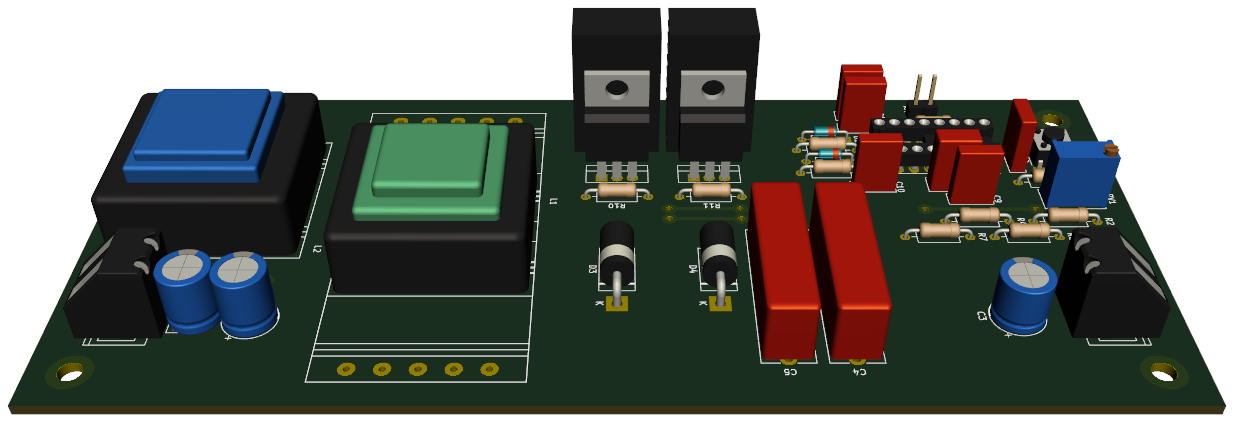
\includegraphics[scale=.35]{pdf/fotos/tecnica_3ssc.png}
        \label{fig:3d_tecnica_3ssc}
     	\indentedfont[15.5cm]{Elaboração própria (2021)}
    \end{figure}
    
    Assim, a \autoref{fig:med_cond_3ssc20k_EG} apresenta a comparação dos resultados obtidos da emissão conduzida para o circuito inicial (CBI) e para a nova estrutura (conversor 3SSC) em uma frequência de \SI{20}{\kilo\hertz}.
    
    \begin{figure}[H]
    	\centering
    	\caption{Comparação dos resultados do ensaio de emissão conduzida para um CBI e um conversor 3SSC com uma frequência de chaveamento de \SI{20}{\kilo\hertz}}
    	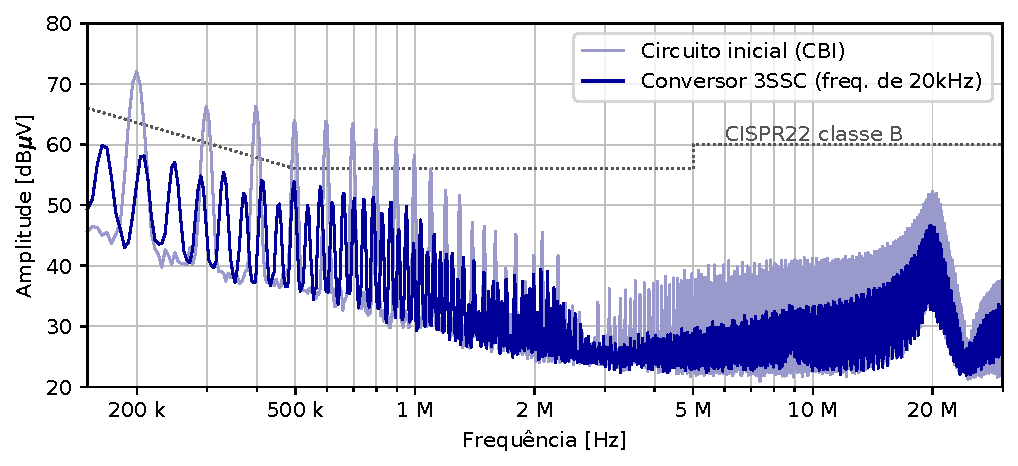
\includegraphics[scale=.9]{pdf/cond/Conversor 3SSC (freq. de 20kHz).pdf}
    	\label{fig:med_cond_3ssc20k_EG}
     	\indentedfont[15.5cm]{Elaboração própria (2021)}
    \end{figure}
    
    Nota-se nesse teste que, diferente das técnicas anteriores, foi possível reduzir consideravelmente os níveis de emissão conduzida em toda a faixa avaliada. 
    
    Na \autoref{fig:med_rad_3ssc20k_EG}, tem-se o comparativo dos resultados da emissão irradiada para o circuito inicial (CBI) e para a nova estrutura (conversor 3SSC) em uma frequência de \SI{20}{\kilo\hertz}.
    
    \begin{figure}[H]
    	\centering
    	\caption{Comparação dos resultados do ensaio de emissão irradiada para um CBI e um conversor 3SSC com uma frequência de chaveamento de \SI{20}{\kilo\hertz}}
    	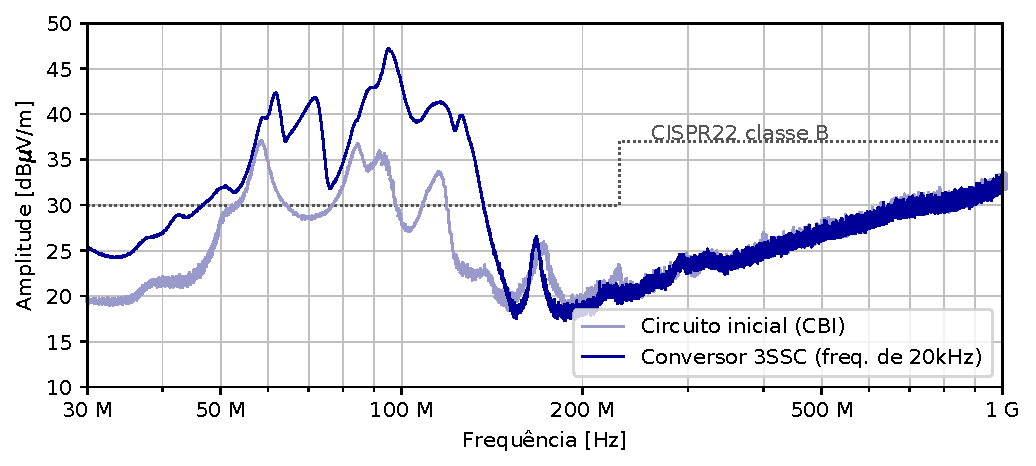
\includegraphics[scale=.9]{pdf/rad/Conversor 3SSC (freq. de 20kHz).pdf}
    	\label{fig:med_rad_3ssc20k_EG}
     	\indentedfont[15.5cm]{Elaboração própria (2021)}
    \end{figure}
    
    Diferente do teste de emissão conduzida, na emissão irradiada, houve um acréscimo nos níveis emitidos, para frequências inferiores \SI{170}{\mega\hertz}. 
    
    Durante os testes, percebeu-se que uma possível causa do aumento nos níveis de irradiação poderia ser o tamanho do entreferro escolhido para o indutor L3. Dessa forma, o indutor foi reprojetado, utilizando um entreferro menor, mantendo o seu valor de indutância. A \autoref{fig:med_cond_3ssc20k} apresenta a comparação dos resultados obtidos da emissão conduzida para o circuito inicial (CBI) e para a nova estrutura (conversor 3SSC) em uma frequência de \SI{20}{\kilo\hertz} para um entreferro reduzido.
    
    \begin{figure}[H]
    	\centering
    	\caption{Comparação dos resultados do ensaio de emissão conduzida para um CBI e um conversor 3SSC com uma frequência de chaveamento de \SI{20}{\kilo\hertz} para um entreferro reduzido}
    	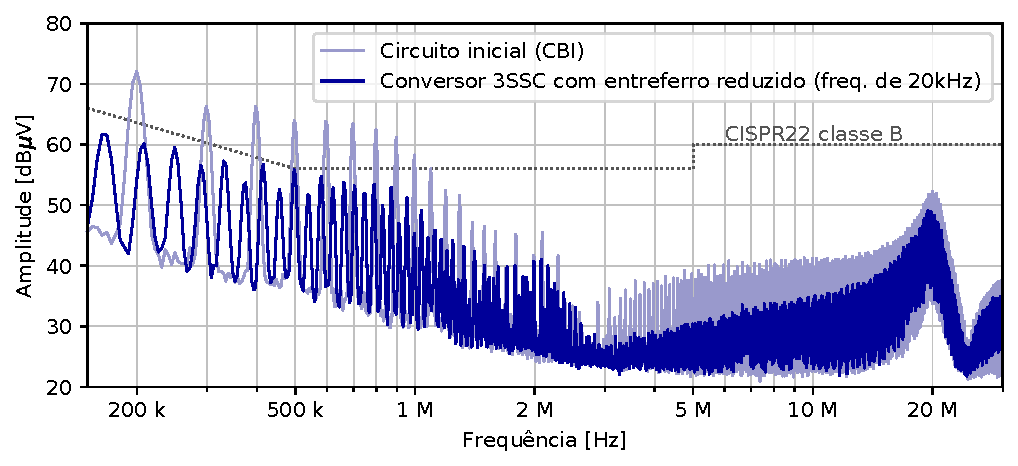
\includegraphics[scale=.9]{pdf/cond/Conversor 3SSC com entreferro reduzido (freq. de 20kHz).pdf}
    	\label{fig:med_cond_3ssc20k}
     	\indentedfont[15.5cm]{Elaboração própria (2021)}
    \end{figure}
    
    Na emissão conduzida não houve grandes mudanças nos resultados entre o entreferro grande e reduzido, como apresentado na \autoref{fig:med_cond_3ssc_comp}, ficando seus valores de pico muito próximos.
    
    \begin{figure}[H]
    	\centering
    	\caption{Comparação dos resultados do ensaio de emissão conduzida entre um conversor 3SSC com uma frequência de chaveamento de \SI{20}{\kilo\hertz} para um entreferro grande e um entreferro reduzido}
    	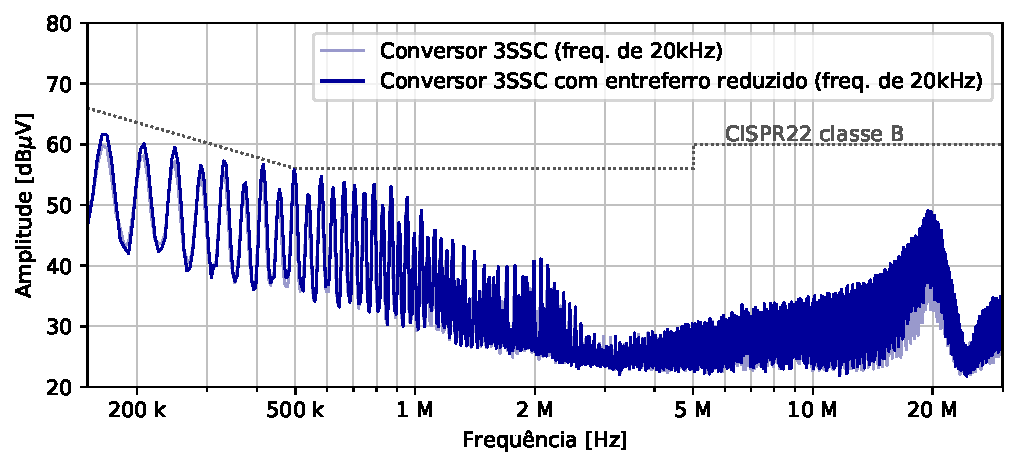
\includegraphics[scale=.9]{pdf/cond/cond-Conversor 3SSC (freq. de 20kHz)-Conversor 3SSC com entreferro reduzido (freq. de 20kHz).pdf}
    	\label{fig:med_cond_3ssc_comp}
     	\indentedfont[15.5cm]{Elaboração própria (2021)}
    \end{figure}
    
    Porém, para a emissão irradiada nos resultados entre o entreferro grande e reduzido, \autoref{fig:med_rad_3ssc20k}, houveram mudanças maiores. 
    
    \begin{figure}[H]
    	\centering
    	\caption{Comparação dos resultados do ensaio de emissão irradiada para um CBI e um conversor 3SSC com uma frequência de chaveamento de \SI{20}{\kilo\hertz} para um entreferro reduzido}
    	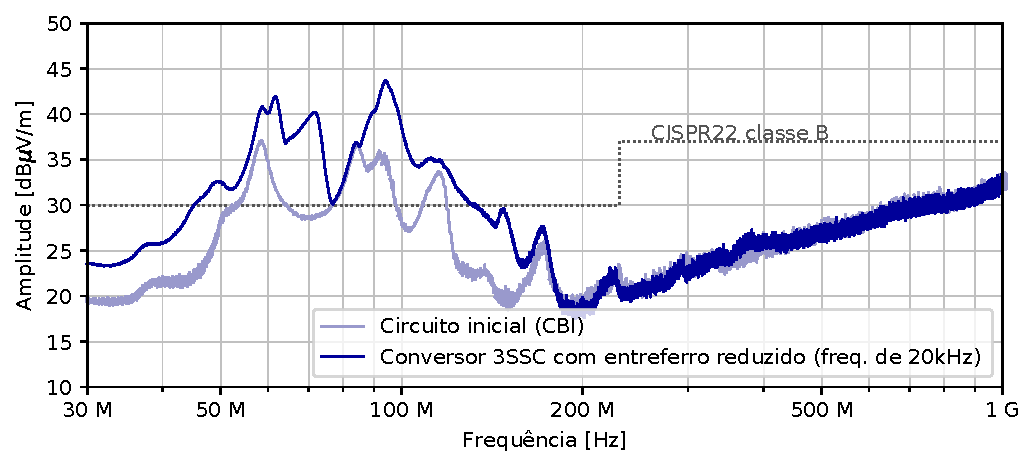
\includegraphics[scale=.9]{pdf/rad/Conversor 3SSC com entreferro reduzido (freq. de 20kHz).pdf}
    	\label{fig:med_rad_3ssc20k}
     	\indentedfont[15.5cm]{Elaboração própria (2021)}
    \end{figure}
    
    Pela figura, percebe-se que, apesar dos maiores picos, se comparado ao CBI inicial, há uma menor emissão irradiada se comparado ao conversor 3SSC com o entreferro grande. Essa diferença entre a emissão irradiada do conversor 3SSC com o indutor com entreferro grande e com o entreferro reduzido pode ser observado na \autoref{fig:med_rad_3ssc_comp}. 
    
    \begin{figure}[H]
    	\centering
    	\caption{Comparação dos resultados do ensaio de emissão irradiada entre um conversor 3SSC com uma frequência de chaveamento de \SI{20}{\kilo\hertz} para um entreferro grande e um entreferro reduzido}
    	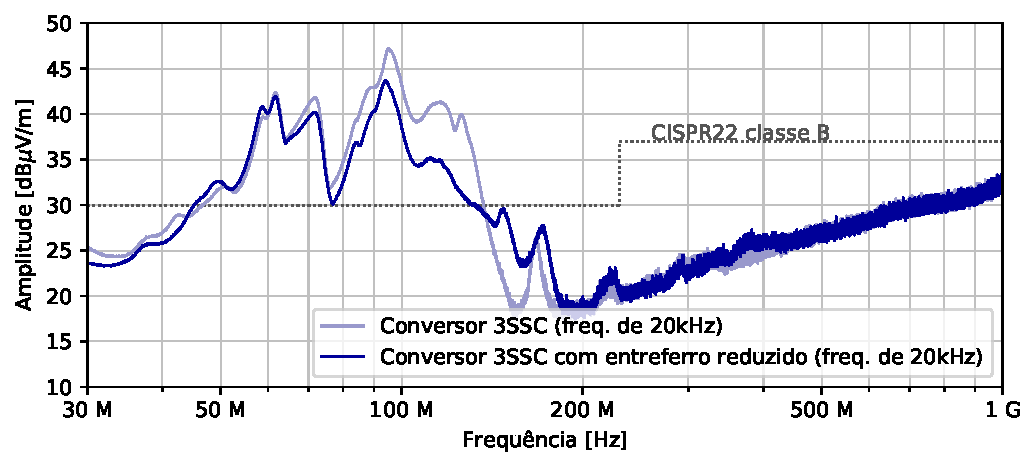
\includegraphics[scale=.9]{pdf/rad/rad-Conversor 3SSC (freq. de 20kHz)-Conversor 3SSC com entreferro reduzido (freq. de 20kHz).pdf}
    	\label{fig:med_rad_3ssc_comp}
     	\indentedfont[15.5cm]{Elaboração própria (2021)}
    \end{figure}
    
    Na figura, nota-se uma redução nos níveis emitidos entre as frequências de \SI{80}{\mega\hertz} e \SI{200}{\mega\hertz} devido a mudança no entreferro do indutor. Assim, apesar da redução nos níveis de emissão conduzida para essa estrutura, há um aumento na emissão irradiada. Ainda, percebe-se a necessidade de um grande cuidado ao projetar os indutores, uma vez que seu entreferro é um dos grandes responsáveis pela emissão irradiada. 
    %%%%%%%%%%%%%%%%%%%%%%%%%%%%%%%%%%%%%%%%%%%%%%%%%%%%%%%%%%%%%%%%%%%
    \subsection{Uso combinado das técnicas com melhores resultados} \label{cap:result_tecnicas_total}
    %%%%%%%%%%%%%%%%%%%%%%%%%%%%%%%%%%%%%%%%%%%%%%%%%%%%%%%%%%%%%%%%%%%
    
    O uso do conversor 3SSC, apesar de apresentar maiores níveis de emissão irradiada, consiste em uma boa alternativa para a redução da emissão conduzida, podendo até substituir o uso de filtros como técnica. Aliado ao conversor 3SSC, algumas técnicas e soluções de mitigação de emissão irradiada podem ser aplicadas, buscando um equilíbrio entre as emissões. 
    
    Assim, buscando demonstrar a viabilidade das técnicas estudadas, aplicou-se uma combinação das técnicas com melhor resultado junto ao conversor 3SSC. Dessa forma, foi utilizado a técnica de uso de um núcleo de ferrite nos terminais de dreno dos transistores e a conexão dos dissipadores á referência do circuito com um capacitor de \SI{100}{\nano\farad}. A \autoref{fig:med_cond_todas_tec} apresenta o comparativo entre os resultados do ensaio de emissão conduzida do circuito inicial (CBI) e o uso das técnicas com melhores resultados (uso de um núcleo de ferrite no terminal de dreno + conexão dos dissipadores à referência + conversor 3SSC com frequência de operação de \SI{20}{\kilo\hertz}).
    
    \begin{figure}[H]
    	\centering
    	\caption{Comparação entre os resultados do ensaio de emissão conduzida do circuito inicial e o uso das técnicas com melhores resultados}
    	\includegraphics[scale=.9]{pdf/cond/Uso das melhores técnicas.pdf}
    	\label{fig:med_cond_todas_tec}
     	\indentedfont[15.5cm]{Elaboração própria (2021)}
    \end{figure}
    
    Percebe-se pela figura, que apesar de não ser o objetivo desse estudo, o uso das técnicas combinadas foram capazes de colocar o conversor proposto abaixo dos níveis estabelecidos pela norma CISPR22 classe B de emissão conduzida. A \autoref{fig:med_rad_todas_tec} apresenta o comparativo da emissão irradiada para o mesmo teste. 
    
    \begin{figure}[H]
    	\centering
    	\caption{Comparação entre os resultados do ensaio de emissão irradiada do circuito inicial e o uso das técnicas com melhores resultados}
    	\includegraphics[scale=.9]{pdf/rad/Uso das melhores técnicas.pdf}s
    	\label{fig:med_rad_todas_tec}
     	\indentedfont[15.5cm]{Elaboração própria (2021)}
    \end{figure}
    
    Um resultado semelhante a emissão conduzida pode ser observado nessa figura, que apesar do aumento na emissão irradiada provocada pelo conversor 3SSC, as demais técnicas utilizadas foram capazes de contrabalancear essa emissão. Percebe-se que há uma grande redução nos níveis medidos em toda a faixa avaliada na norma, com apenas alguns poucos pontos acima dos limites estabelecidos por ela. 
    